%!TEX root = ../main.tex
\chapter{Elementi di dinamica del corpo rigido}

\section{Il corpo rigido}

\subsection{Definizione e osservazioni generali}
Un corpo rigido è un corpo che non può più essere approssimato a un punto materiale ma che ha una certa estensione. Il fatto che sia rigido comporta assenza di movimento delle parti interne del sistema. Esso si può immaginare come un particolare sistema di punti materiali semplificato. In questo caso si va a suddividere il corpo esteso in tante particelle molto piccole di massa infinitesima $dm$ che andranno a sostituire le masse $i$-esime.

\begin{figure}[htpb]
	\centering

	\tikzset{every picture/.style={line width=0.75pt}} %set default line width to 0.75pt        

	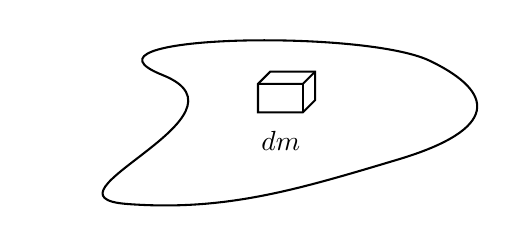
\begin{tikzpicture}[x=0.75pt,y=0.75pt,yscale=-1,xscale=1]
	%uncomment if require: \path (0,300); %set diagram left start at 0, and has height of 300

	%Shape: Polygon Curved [id:ds9077710605730196] 
	\draw   (221,83.31) .. controls (172.5,64) and (317.5,61) .. (349.66,76.41) .. controls (381.83,91.82) and (383.12,109.45) .. (334.5,124) .. controls (285.88,138.55) and (251.5,149) .. (204.01,145.45) .. controls (156.52,141.91) and (269.51,102.63) .. (221,83.31) -- cycle ;
	%Shape: Cube [id:dp5839980293890457] 
	\draw   (267,87.58) -- (272.88,81.7) -- (294.5,81.7) -- (294.5,95.42) -- (288.62,101.3) -- (267,101.3) -- cycle ; \draw   (294.5,81.7) -- (288.62,87.58) -- (267,87.58) ; \draw   (288.62,87.58) -- (288.62,101.3) ;

	% Text Node
	\draw (278,115) node    {$dm$};

	\end{tikzpicture}
\end{figure}
\FloatBarrier
Infatti, invece di utilizzare il concetto di sommatoria si ha quello di somma continua, che non è altro che l'integrale esteso all'intero volume del corpo, o esteso alla superficie o esteso alla linea, se il corpo è approssimabile a una superficie o a una linea.

Mentre quando si aveva il sistema di punti materiali, in generale una massa si poteva muovere rispetto all'altra, nel corpo rigido ciò non avviene. Si richiamano le equazioni cardinali della dinamica definite per un sistema di punti materiali:

\[
	\boxed{\vec{R}_{est} = M_{tot}\cdot \vec{a}_{cm} \qquad \vec{M}^{(o)}_{est} = \frac{d\vec{L}^{(o)}_{tot}}{dt} \qquad \mathcal{L}_{int} + \mathcal{L}_{est} = \Delta E_{K,tot}   }
\]

Queste relazioni sono applicabili al corpo rigido. Le forze interne in esso non compiono mai lavoro perché vista la rigidità, non mettono in movimento nessuna parte dell'oggetto. Quindi le uniche forze che vanno considerate sono quelle esterne. La seconda semplificazione è che se in un sistema di punti materiali si hanno molti gradi di libertà,  un corpo rigido è caratterizzato da $6$ di essi. Infatti, dato che questo corpo non si deforma, lo si definisce andando a individuare la posizione di un punto. A questo punto il corpo può ancora muoversi rispetto ad esso, per questo gli si conferisce un angolo di rotazione rispetto ai tre assi. Assegnare un angolo di rotazione e la posizione di un punto, significa individuare $3+3=6$ coordinate nello spazio. \emph{Se il sistema è definito da $6$ gradi di libertà, servono solo sei equazioni scalari per conoscere completamente il moto complessivo del corpo rigido}. Esse sono date dalla prima e la seconda equazione cardinale della dinamica. Questo primo risultato conferma l'osservazione che il moto di un corpo rigido è più complesso di quello di un punto materiale.

\paragraph{Osservazione} Indicati con $l$ i gradi di libertà, così come per un corpo rigido si ha $l=6$, si noti che:

\begin{itemize}
	\item un punto materiale avrà $l=3$;
	\item $n$ punti materiali indipendenti avranno $l=3n$;
	\item un punto vincolato a muoversi lungo una linea avrà $l=1$, sopra una superficie avrà invece $l=2$;
	\item due punti vincolati ad avere sempre la stessa distanza fra loro avranno $l=5$.
\end{itemize}

Si risolve quindi completamente il sistema andando a studiare l'effetto della risultante delle forze e dei momenti delle forze. Il teorema dell'energia cinetica può essere sostituito a una delle sei relazioni scalari per studiare eventualmente in maniera più semplice il moto del corpo dal punto di vista energetico.

\subsection{Il centro di massa nel corpo rigido}

A questo punto si può andare a capire cosa vuol dire passare da una notazione con la sommatoria a una con l'integrale. Si consideri un corpo rigido di forma qualunque. L'obbiettivo è quello di calcolare la posizione di $cm$ rispetto alla posizione di un certo osservatore $O$. Si è definito il centro di massa come:

\[
	\vec{r}_\text{CM} = \frac{\sum_i m_i r_i}{M}
\]

Ora si approssima il corpo e lo si vede come costituito da tanti volumetti infinitesimi.

\begin{figure}[htpb]
	\centering

	\tikzset{every picture/.style={line width=0.75pt}} %set default line width to 0.75pt        

	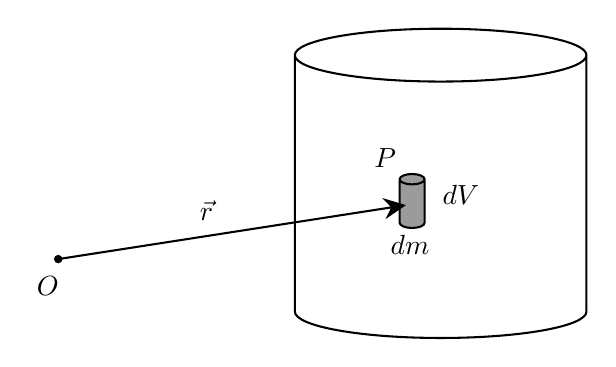
\begin{tikzpicture}[x=0.75pt,y=0.75pt,yscale=-1,xscale=1]
	%uncomment if require: \path (0,300); %set diagram left start at 0, and has height of 300

	%Shape: Can [id:dp03669144619399156] 
	\draw   (366.5,76.73) -- (366.5,200.27) .. controls (366.5,207.3) and (335.05,213) .. (296.25,213) .. controls (257.45,213) and (226,207.3) .. (226,200.27) -- (226,76.73) .. controls (226,69.7) and (257.45,64) .. (296.25,64) .. controls (335.05,64) and (366.5,69.7) .. (366.5,76.73) .. controls (366.5,83.76) and (335.05,89.46) .. (296.25,89.46) .. controls (257.45,89.46) and (226,83.76) .. (226,76.73) ;
	%Shape: Can [id:dp6672302852048766] 
	\draw  [fill={rgb, 255:red, 155; green, 155; blue, 155 }  ,fill opacity=1 ] (288.5,136.5) -- (288.5,157.5) .. controls (288.5,158.88) and (285.81,160) .. (282.5,160) .. controls (279.19,160) and (276.5,158.88) .. (276.5,157.5) -- (276.5,136.5) .. controls (276.5,135.12) and (279.19,134) .. (282.5,134) .. controls (285.81,134) and (288.5,135.12) .. (288.5,136.5) .. controls (288.5,137.88) and (285.81,139) .. (282.5,139) .. controls (279.19,139) and (276.5,137.88) .. (276.5,136.5) ;
	%Straight Lines [id:da1696202666868456] 
	\draw    (112,175) -- (276.54,149.46) ;
	\draw [shift={(279.5,149)}, rotate = 531.1800000000001] [fill={rgb, 255:red, 0; green, 0; blue, 0 }  ][line width=0.08]  [draw opacity=0] (10.72,-5.15) -- (0,0) -- (10.72,5.15) -- (7.12,0) -- cycle    ;
	%Shape: Circle [id:dp9601969907529446] 
	\draw  [fill={rgb, 255:red, 0; green, 0; blue, 0 }  ,fill opacity=1 ] (110.5,175) .. controls (110.5,174.17) and (111.17,173.5) .. (112,173.5) .. controls (112.83,173.5) and (113.5,174.17) .. (113.5,175) .. controls (113.5,175.83) and (112.83,176.5) .. (112,176.5) .. controls (111.17,176.5) and (110.5,175.83) .. (110.5,175) -- cycle ;

	% Text Node
	\draw (281.5,168) node    {$dm$};
	% Text Node
	\draw (306,144) node    {$dV$};
	% Text Node
	\draw (107,188) node    {$O$};
	% Text Node
	\draw (183.5,151.5) node    {$\vec{r}$};
	% Text Node
	\draw (269.5,126.5) node    {$P$};

	\end{tikzpicture}
\end{figure}
\FloatBarrier

\[
	\vec{r}_\text{CM} = \frac{\int_{\text{volume}} dm\,\vec{r} (P)}{M}
\]
$\vec{r} (P)$ non è costante ma è funzione della posizione. Andare a ricoprire in maniera continua il volume, significa fare una somma continua su tutto il volume, quello che si chiama \emph{integrale di volume}, o \emph{integrale triplo}.

\[
	\int_{\text{volume}} = \iiint
\]

In generale i corpi rigidi non sono copri omogenei, la massa non è distribuita in maniera uniforme sul volume del corpo. Per dare questa informazione si introduce il concetto di \textbf{densità volumetrica}, ovvero il rapporto tra la massa infinitesima del corpo e il volumetto infinitesimo $dV$.

\[
	\rho = \frac{dm}{dV}
\]

Nota questa grandezza, che dimensionalmente è una massa su una lunghezza al cubo e si misurerà in $kg/m^3$, si può andare a introdurla dentro alla definizione di centro di massa: invece di scrivere $dm$, la si sostituisce con la densità per il volumetto infinitesimo.

\[
	\vec{r}_\text{CM} = \frac{\int_{\text{volume}}\rho (P)\, \vec{r} (P)\, dr}{M}
\]

La variabile di integrazione è il volumetto infinitesimo, per ognuno di essi bisogna valutare quanto vale il prodotto fra la densità del corpo in quel punto e il vettore posizione che ne identifica la posizione. Questa diventa le definizione di posizione del centro di massa per un corpo tridimensionale. Se il corpo è omogeneo, $\rho$ è costante e sarà pari a $M/V$. Si ha in tal caso:

\[
	\vec{r}_\text{CM} = \rho \frac{\int_{\text{volume}}\vec{r} (P)dV }{M} = \frac{M}{V} \frac{\int_{\text{volume}}\vec{r} (P)dV }{M} = \frac{\int_{\text{volume}}\vec{r} (P)dV }{V}
\]

Questa definizione può essere estesa al caso in cui il corpo invece che essere tridimensionale, è approssimabile a una superficie.

\begin{figure}[htpb]
	\centering

	\tikzset{every picture/.style={line width=0.75pt}} %set default line width to 0.75pt        

	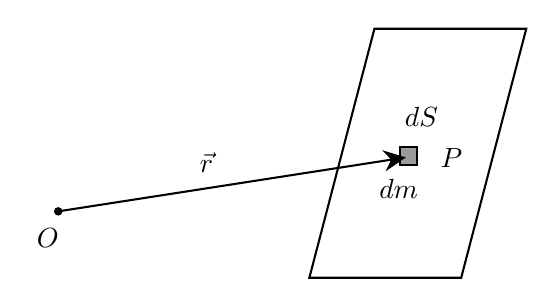
\begin{tikzpicture}[x=0.75pt,y=0.75pt,yscale=-1,xscale=1]
	%uncomment if require: \path (0,300); %set diagram left start at 0, and has height of 300

	%Shape: Parallelogram [id:dp9250279294336241] 
	\draw   (276.35,92) -- (349.5,92) -- (318.15,212) -- (245,212) -- cycle ;
	%Shape: Square [id:dp3084993720003819] 
	\draw  [fill={rgb, 255:red, 155; green, 155; blue, 155 }  ,fill opacity=1 ] (288.5,149) -- (297,149) -- (297,157.5) -- (288.5,157.5) -- cycle ;
	%Straight Lines [id:da7733792598985865] 
	\draw    (124,180) -- (288.54,154.46) ;
	\draw [shift={(291.5,154)}, rotate = 531.1800000000001] [fill={rgb, 255:red, 0; green, 0; blue, 0 }  ][line width=0.08]  [draw opacity=0] (10.72,-5.15) -- (0,0) -- (10.72,5.15) -- (7.12,0) -- cycle    ;
	%Shape: Circle [id:dp06205929212849104] 
	\draw  [fill={rgb, 255:red, 0; green, 0; blue, 0 }  ,fill opacity=1 ] (122.5,180) .. controls (122.5,179.17) and (123.17,178.5) .. (124,178.5) .. controls (124.83,178.5) and (125.5,179.17) .. (125.5,180) .. controls (125.5,180.83) and (124.83,181.5) .. (124,181.5) .. controls (123.17,181.5) and (122.5,180.83) .. (122.5,180) -- cycle ;

	% Text Node
	\draw (299,134.5) node    {$dS$};
	% Text Node
	\draw (288,169) node    {$dm$};
	% Text Node
	\draw (119,193) node    {$O$};
	% Text Node
	\draw (195.5,156.5) node    {$\vec{r}$};
	% Text Node
	\draw (313.5,154.5) node    {$P$};

	\end{tikzpicture}
\end{figure}
\FloatBarrier
Si divide il corpo in tanti elementi $m_i$ infinitesimi in cui la superficie è $dS$ e si introduce il concetto di \textbf{densità superficiale}, $\sigma$, che non è altro che il rapporto tra la massa infinitesima e l'elementino di superficie infinitesimo.

\[
	\sigma=\frac{dm}{dS}
\]

Riprendendo la definizione data del vettore posizione del centro di massa, la somma continua è un \emph{integrale di superficie} dove al posto di $dm$ si può sostituire $\sigma \,dS$. L'elemento di integrazione è $dS$.

\[
	\vec{r}_\text{CM} = \frac{\int_{\text{superficie}}\vec{r} (P) \sigma(P) dS}{M}
	\]

Se però il corpo è omogeneo:

\[
	\vec{r}_\text{CM} = \frac{M}{S} \frac{\int_{\text{superficie}}\vec{r} (P)dS}{M} = \frac{\int_{\text{superficie}}\vec{r} (P)dS}{S}
\]

Infine si può considerare il caso in cui il corpo rigido può essere approssimato ad una linea.

\begin{figure}[htpb]
	\centering

	\tikzset{every picture/.style={line width=0.75pt}} %set default line width to 0.75pt        

	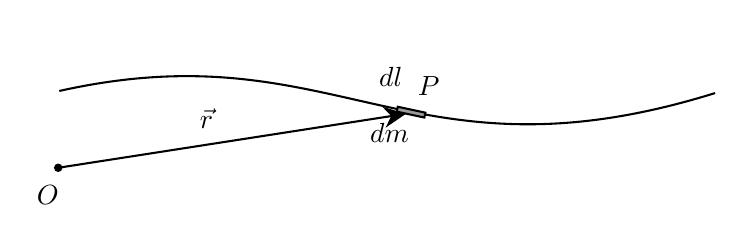
\begin{tikzpicture}[x=0.75pt,y=0.75pt,yscale=-1,xscale=1]
	%uncomment if require: \path (0,300); %set diagram left start at 0, and has height of 300

	%Curve Lines [id:da02030950644760532] 
	\draw    (98.5,124) .. controls (232.5,94) and (266.5,171) .. (414.5,125) ;
	%Shape: Rectangle [id:dp3105990545838513] 
	\draw  [fill={rgb, 255:red, 155; green, 155; blue, 155 }  ,fill opacity=1 ] (261.6,131.6) -- (274.9,134.45) -- (274.4,136.8) -- (261.1,133.95) -- cycle ;
	%Straight Lines [id:da07326605801202035] 
	\draw    (98,161) -- (262.54,135.46) ;
	\draw [shift={(265.5,135)}, rotate = 531.1800000000001] [fill={rgb, 255:red, 0; green, 0; blue, 0 }  ][line width=0.08]  [draw opacity=0] (10.72,-5.15) -- (0,0) -- (10.72,5.15) -- (7.12,0) -- cycle    ;
	%Shape: Circle [id:dp4453267725448391] 
	\draw  [fill={rgb, 255:red, 0; green, 0; blue, 0 }  ,fill opacity=1 ] (96.5,161) .. controls (96.5,160.17) and (97.17,159.5) .. (98,159.5) .. controls (98.83,159.5) and (99.5,160.17) .. (99.5,161) .. controls (99.5,161.83) and (98.83,162.5) .. (98,162.5) .. controls (97.17,162.5) and (96.5,161.83) .. (96.5,161) -- cycle ;

	% Text Node
	\draw (257.6,144) node    {$dm$};
	% Text Node
	\draw (258.2,117.2) node    {$dl$};
	% Text Node
	\draw (93,174) node    {$O$};
	% Text Node
	\draw (169.5,137.5) node    {$\vec{r}$};
	% Text Node
	\draw (276.5,121.5) node    {$P$};

	\end{tikzpicture}
\end{figure}
\FloatBarrier
In tali casi, si va a suddividere la linea in tanti elementini di linea infinitesimi. Si definisce una \textbf{densità lineare} come il rapporto tra la massa infinitesima e la lunghezza $dl$.

\[
	\lambda (P)= \frac{dm}{dl}
\]

Ovviamente questa grandezza è una massa su una lunghezza.

\[
	\vec{r}_\text{CM} = \frac{\int_{\text{linea} }dm\,\vec{r} (P) }{M} =\vec{r}_\text{CM} = \frac{\int_{\text{linea} }\lambda(P)\,\vec{r} (P)\, dl}{M}
\]

Se il corpo è omogeneo, la densità lineare si può considerare come costante in ogni punto del corpo ed è data da il rapporto fra la massa e la sua lunghezza. Allora la definizione di vettore posizione del centro di massa sarà:

\[
	\vec{r}_\text{CM} = \frac{M}{L} \frac{\int_{\text{linea} }\vec{r} (P) dl}{M} = \frac{\int_{\text{linea} }\vec{r} (P) dl}{L}
\]

Se un corpo omogeneo è simmetrico rispetto ad un punto, un asse o un piano, il centro di massa rispettivamente coincide col centro di simmetria o è un punto dell'asse o del piano di simmetria. Se esistono più assi o piani di simmetria, il centro di massa sta sulla loro intersezione.

Si consideri un'asta rigida a forma di semi anello di raggio $R$, di densità uniforme.

\begin{figure}[htpb]
	\centering

	\tikzset{every picture/.style={line width=0.75pt}} %set default line width to 0.75pt        

	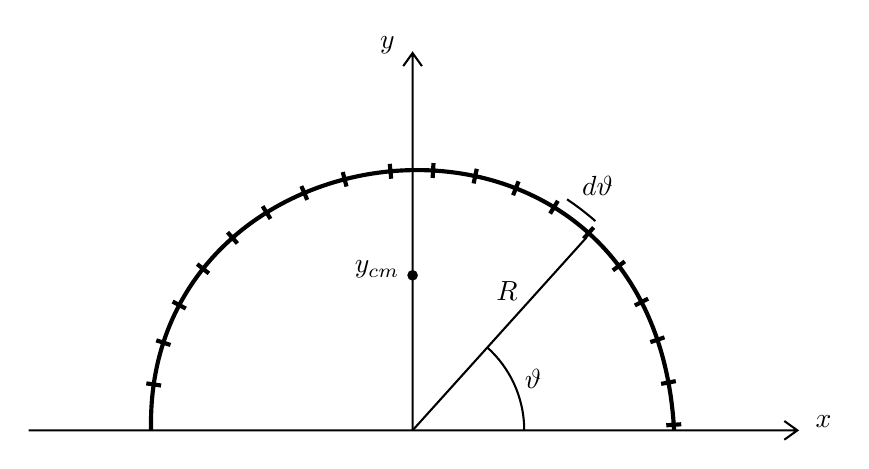
\begin{tikzpicture}[x=0.75pt,y=0.75pt,yscale=-0.9,xscale=0.9]
	%uncomment if require: \path (0,300); %set diagram left start at 0, and has height of 300

	%Shape: Axis 2D [id:dp20288318873505573] 
	\draw  (68,241.25) -- (479.5,241.25)(273.5,39.25) -- (273.5,241.25) (472.5,236.25) -- (479.5,241.25) -- (472.5,246.25) (268.5,46.25) -- (273.5,39.25) -- (278.5,46.25)  ;
	%Curve Lines [id:da27128963796582406] 
	\draw [color={rgb, 255:red, 0; green, 0; blue, 0 }  ,draw opacity=1 ][line width=1.5]    (133.5,241.25) .. controls (129.5,70.25) and (402.5,41.25) .. (413.5,241.25)(130.95,216.11) -- (138.87,217.24)(136.27,193.06) -- (143.88,195.53)(145.04,172.31) -- (152.11,176.05)(158.19,152.25) -- (164.45,157.23)(174.44,135.2) -- (179.73,141.2)(193.21,121.25) -- (197.44,128.04)(213.96,110.48) -- (217.09,117.85)(236.12,102.98) -- (238.12,110.72)(261.29,98.59) -- (262.03,106.56)(284.69,98.16) -- (284.24,106.14)(307.85,101.24) -- (306.18,109.07)(330.24,107.95) -- (327.31,115.4)(351.29,118.39) -- (347.12,125.22)(370.43,132.64) -- (365.08,138.59)(387.1,150.8) -- (380.72,155.63)(399.6,170.73) -- (392.49,174.39)(408.35,191.47) -- (400.77,194.03)(414.4,214.9) -- (406.54,216.37)(417.31,237.99) -- (409.32,238.54) ;
	%Shape: Circle [id:dp81385918280685] 
	\draw  [fill={rgb, 255:red, 0; green, 0; blue, 0 }  ,fill opacity=1 ] (271.25,158.25) .. controls (271.25,157.01) and (272.26,156) .. (273.5,156) .. controls (274.74,156) and (275.75,157.01) .. (275.75,158.25) .. controls (275.75,159.49) and (274.74,160.5) .. (273.5,160.5) .. controls (272.26,160.5) and (271.25,159.49) .. (271.25,158.25) -- cycle ;
	%Straight Lines [id:da1883230978266146] 
	\draw    (273.5,241.25) -- (366.67,137.92) ;
	%Shape: Arc [id:dp5171778667888058] 
	\draw  [draw opacity=0] (313.36,196.74) .. controls (325.52,207.64) and (333.2,223.45) .. (333.25,241.06) -- (273.5,241.25) -- cycle ; \draw   (313.36,196.74) .. controls (325.52,207.64) and (333.2,223.45) .. (333.25,241.06) ;
	%Shape: Arc [id:dp10120721800348642] 
	\draw  [draw opacity=0] (356.19,117.58) .. controls (361.5,121.14) and (366.57,125.03) .. (371.36,129.22) -- (273.5,241.25) -- cycle ; \draw   (356.19,117.58) .. controls (361.5,121.14) and (366.57,125.03) .. (371.36,129.22) ;

	% Text Node
	\draw (254.5,155.25) node    {$y_{cm}$};
	% Text Node
	\draw (372.5,110.25) node    {$d\vartheta $};
	% Text Node
	\draw (338,213.75) node    {$\vartheta $};
	% Text Node
	\draw (493.5,236.75) node    {$x$};
	% Text Node
	\draw (260,35.25) node    {$y$};
	% Text Node
	\draw (324,166.75) node    {$R$};

	\end{tikzpicture}
\end{figure}
\FloatBarrier
Si avrà:

\[
	\lambda = \frac{M}{\pi R}
\]

Si posiziona l'origine sul centro della circonferenza e si fissano due assi $x$ e $y$. Per ragioni di simmetria il baricentro dovrà per forza appartenere all'asse $y$. L'ascissa del centro di massa va a $0$. Se ne calcola l'ordinata:

\[
	\vec{r}_\text{CM} = \frac{\int_{\text{linea} } \vec{r} (P)dl}{L} \qquad y_{cm}=\frac{\int_{\text{linea} }y(P)dl}{L} = \frac{1}{\pi R} \int_{\text{linea} } y(P) dl
\]

Operare un integrale di linea vuol dire andarla a suddividere in tanti segmentini infinitesimi di lunghezza $dl$. Tutte le volte che si ha un corpo dalla forma caratterizzata da una certa simmetria radiale, conviene andare a lavorare con le coordinate radiali. Bisogna trasformare quell'integrale nella nuova variabile di integrazione angolare.
$dl$ in questo caso è il solito arco di circonferenza di ampiezza $d\vartheta$, $dl=R\,d\vartheta$

\[
	\frac{1}{\pi R}\int_{\text{linea}} y(R)Rd\vartheta = \frac{1}{\pi R}\int_{0\text{ linea} }^{\pi } \sin \vartheta R^2 d\vartheta = \frac{R}{\pi }[-\cos \vartheta ]_0^{\pi } = \frac{2R}{\pi}
\]

\subsection{Punto di applicazione di una forza}

Essendo il corpo esteso, si dovrà porre particolare attenzione al \emph{punto di applicazione della forza}, problema che non si presentava per il punto materiale. Se si ha una singola forza che spinge o che tira in un punto, il punto di applicazione coincide esso. Esistono tuttavia anche delle forze distribuite su tutto il corpo, come la \textbf{forza peso}. È necessario quindi calcolare la forza peso totale, capire quanto vale e dove applicarla.
Considerare la forza peso totale, significa fare la somma di tutte le forze peso associate alle masse infinitesime:

\[
	\vec{F}_{peso,tot} = \sum_i m_i\vec{g} = \int dm\,\vec{g} = \vec{g} \int dm = M\vec{g}
\]

Si calcola invece il momento totale rispetto ad un generico polo generato dalla forza peso:

\[
	\vec{M}^{(o)}_{F\,peso} = \sum_i \vec{r}_i \times m_i\,\vec{g} = \int_{\text{corpo}}\vec{r} (P)\times \vec{g} \,dm
\]

Si ha di nuovo che $\vec{g}$ è la stessa per tutti i termini e può essere portata fuori dall'integrale. Si ritrova così un integrale che coincide con il vettore posizione del centro di massa per la massa del corpo rigido.

\[
	M\left( \frac{\int\vec{r} (P)dm}{M} \right) \times \vec{g} = \vec{r}_{cm}^{(o)}\cdot M \times \vec{g} = \vec{r}_\text{CM}^{(o)} \times M\vec{g}
\]

Invece che dover calcolare l'azione di tante forze peso infinitesime,  è equivalente trovare il baricentro del corpo ed applicarci la forza peso.

Vi è in realtà un'altra forza distribuita per la quale a priori non è noto il punto di applicazione. Si supponga di avere un corpo appoggiato su un piano d'appoggio, esso sarà soggetto alla forza peso diretta verso il basso.

\begin{figure}[htpb]
	\centering

	\tikzset{every picture/.style={line width=0.75pt}} %set default line width to 0.75pt        

	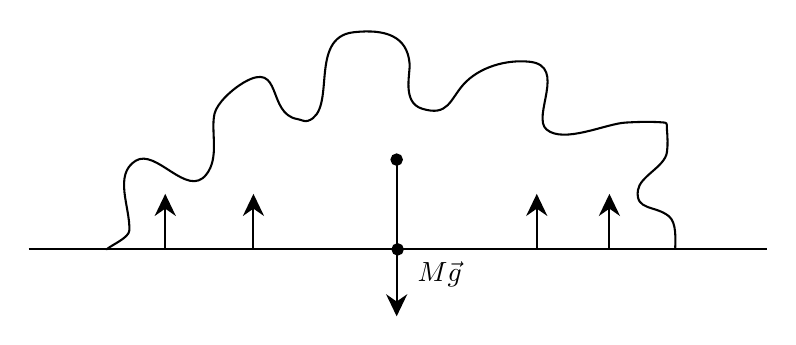
\begin{tikzpicture}[x=0.75pt,y=0.75pt,yscale=-1,xscale=1]
	%uncomment if require: \path (0,300); %set diagram left start at 0, and has height of 300

	%Straight Lines [id:da7441220630131655] 
	\draw    (136,205) -- (491.5,205) ;
	%Curve Lines [id:da6787839247003224] 
	\draw [color={rgb, 255:red, 0; green, 0; blue, 0 }  ][line width=0.75] [line join = round][line cap = round]   (173.5,205) .. controls (176.3,202.66) and (184.38,199.39) .. (184.5,195.8) .. controls (184.87,184.61) and (176.8,169.04) .. (187.5,162.32) .. controls (197.44,156.09) and (212.35,180.51) .. (221.5,169.02) .. controls (228.07,160.77) and (223.59,148.26) .. (225.5,139.73) .. controls (226.67,134.5) and (234.11,127.83) .. (239.5,124.67) .. controls (258.62,113.47) and (250.54,139.74) .. (265.5,142.24) .. controls (267.17,142.52) and (268.92,143.61) .. (270.5,143.08) .. controls (284.86,138.27) and (270.39,102.87) .. (292.5,100.4) .. controls (307.82,98.69) and (318.37,102.18) .. (319.5,115.46) .. controls (319.92,120.43) and (315.72,134.15) .. (325.5,137.22) .. controls (338.13,141.18) and (338.98,132.78) .. (345.5,125.51) .. controls (352.75,117.42) and (365.79,113.32) .. (377.5,114.63) .. controls (395.49,116.64) and (378.12,141.09) .. (385.5,147.26) .. controls (393.78,154.19) and (414.04,144.46) .. (423.5,143.92) .. controls (429.82,143.55) and (436.2,143.36) .. (442.5,143.92) .. controls (443.87,144.04) and (443.41,146.11) .. (443.5,147.26) .. controls (443.79,150.88) and (443.98,154.54) .. (443.5,158.14) .. controls (442.55,165.26) and (430.41,169.71) .. (429.5,176.55) .. controls (428.17,186.54) and (437.99,183.65) .. (444.5,189.1) .. controls (448.25,192.24) and (447.5,200.4) .. (447.5,204.16) ;
	%Straight Lines [id:da19958187671322225] 
	\draw    (201.78,205.26) -- (201.78,181.26) ;
	\draw [shift={(201.78,178.26)}, rotate = 450] [fill={rgb, 255:red, 0; green, 0; blue, 0 }  ][line width=0.08]  [draw opacity=0] (10.72,-5.15) -- (0,0) -- (10.72,5.15) -- (7.12,0) -- cycle    ;
	%Straight Lines [id:da8361420970725475] 
	\draw    (244.28,205.26) -- (244.28,181.26) ;
	\draw [shift={(244.28,178.26)}, rotate = 450] [fill={rgb, 255:red, 0; green, 0; blue, 0 }  ][line width=0.08]  [draw opacity=0] (10.72,-5.15) -- (0,0) -- (10.72,5.15) -- (7.12,0) -- cycle    ;
	%Straight Lines [id:da07338761902668622] 
	\draw    (380.78,205.26) -- (380.78,181.26) ;
	\draw [shift={(380.78,178.26)}, rotate = 450] [fill={rgb, 255:red, 0; green, 0; blue, 0 }  ][line width=0.08]  [draw opacity=0] (10.72,-5.15) -- (0,0) -- (10.72,5.15) -- (7.12,0) -- cycle    ;
	%Straight Lines [id:da18986830705750823] 
	\draw    (415.78,205.26) -- (415.78,181.26) ;
	\draw [shift={(415.78,178.26)}, rotate = 450] [fill={rgb, 255:red, 0; green, 0; blue, 0 }  ][line width=0.08]  [draw opacity=0] (10.72,-5.15) -- (0,0) -- (10.72,5.15) -- (7.12,0) -- cycle    ;
	%Straight Lines [id:da14510448793214303] 
	\draw    (313.28,161.76) -- (313.28,234.26) ;
	\draw [shift={(313.28,237.26)}, rotate = 270] [fill={rgb, 255:red, 0; green, 0; blue, 0 }  ][line width=0.08]  [draw opacity=0] (10.72,-5.15) -- (0,0) -- (10.72,5.15) -- (7.12,0) -- cycle    ;
	%Shape: Circle [id:dp24028553452436285] 
	\draw  [fill={rgb, 255:red, 0; green, 0; blue, 0 }  ,fill opacity=1 ] (310.78,161.76) .. controls (310.78,160.38) and (311.9,159.26) .. (313.28,159.26) .. controls (314.66,159.26) and (315.78,160.38) .. (315.78,161.76) .. controls (315.78,163.14) and (314.66,164.26) .. (313.28,164.26) .. controls (311.9,164.26) and (310.78,163.14) .. (310.78,161.76) -- cycle ;
	%Shape: Circle [id:dp5831623738284168] 
	\draw  [fill={rgb, 255:red, 0; green, 0; blue, 0 }  ,fill opacity=1 ] (311.25,205) .. controls (311.25,203.62) and (312.37,202.5) .. (313.75,202.5) .. controls (315.13,202.5) and (316.25,203.62) .. (316.25,205) .. controls (316.25,206.38) and (315.13,207.5) .. (313.75,207.5) .. controls (312.37,207.5) and (311.25,206.38) .. (311.25,205) -- cycle ;

	% Text Node
	\draw (334,217) node    {$M\vec{g}$};

	\end{tikzpicture}
\end{figure}
\FloatBarrier
Sicuramente il piano d'appoggio genererà una forza di \textbf{reazione normale} a tale piano. Ogni punto di esso è soggetto a una certa reazione normale e quella complessiva è la somma di tutte queste forze. Si troveranno tanti vettori paralleli il cui punto di applicazione è a priori non noto. Si può dimostrare che la reazione normale in questo caso giace nel punto del piano d'appoggio passante per la verticale del centro di massa. Bisogna imporre che il corpo sia fermo, quindi che la risultante delle forze esterne sia nulla.

\[
	R_n-Mg=0
\]

Si impone poi che il corpo non ruoti: rispetto ad un certo polo i momenti delle forze sono uguali a zero. Come polo si sceglie il punto sul piano d'appoggio passante per la verticale.

\[
	M^{(o)} = R_n x = Mgx =0 \implies x=0
\]

La forza peso rispetto al polo non genera momento perché il raggio vettore è diretto parallelamente ad essa e si ha solo un effetto di compressione. Se si immagina di congiungere il punto di applicazione della forza con il polo tramite un'asta rigida e l'asta rigida con la forza che sta agendo, si ottiene un effetto di rotazione. Si ha che la reazione normale genererà un momento concorde all'asse $z$ di intensità pari a $R_n\,\cdot x$.
Perché esso sia zero, bisogna necessariamente avere $x=0$. Se oltre al peso dell'oggetto si applica su di esso una forza che lo schiaccia verso il basso ma in una parte di destra, la porzione in questa zona del piano d'appoggio deve reagire con una reazione normale più intesa tale per cui, in presenza di $F_o$ e della forza peso, la risultante della reazione normale si sposti verso destra per permettere al corpo di rimanere in equilibrio.

\section{Statica del corpo rigido}

Tutte queste informazioni servono per affrontare lo studio del corpo rigido, che si suddivide in statica e in dinamica.
Studiare la statica del corpo corpo rigido è importante perché dà le basi della statica di tutte le strutture. Si tratta di studiare quali sono le posizioni per cui un corpo, se inizialmente fermo, rimane tale. Ciò accade \textit{in primis} se la risultante di tutte le forze che agiscono su di esso si bilanciano. Questa condizione è \emph{necessaria ma non è sufficiente}. L'altra da aggiungere è che i momenti di tutte le forze agenti sul corpo rigido rispetto ad un certo polo si bilancino. Si può dimostrare che se la risultante delle forze è uguale a $0$ allora la sommatoria dei momenti di tutte le forze rispetto a un polo è uguale alla somma dei momenti delle forze rispetto a un altro polo.

\paragraph{Esempio} Si immagini di avere una stanza con un pavimento orizzontale e una parete verticale (come tutte le normali stanze).

\begin{figure}[htpb]
	\centering

	\tikzset{every picture/.style={line width=0.75pt}} %set default line width to 0.75pt        

	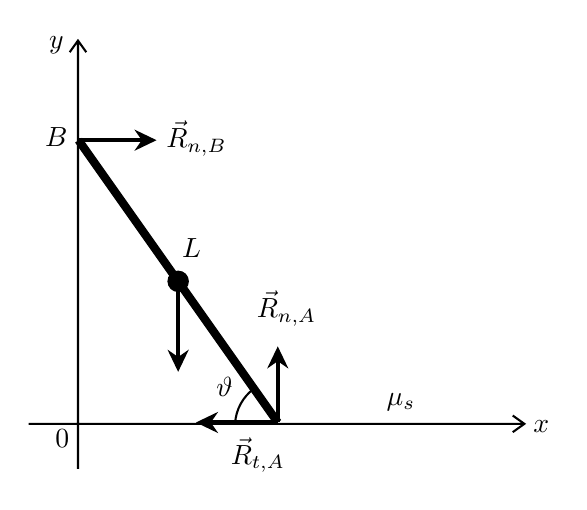
\begin{tikzpicture}[x=0.75pt,y=0.75pt,yscale=-0.8,xscale=0.8]
	%uncomment if require: \path (0,300); %set diagram left start at 0, and has height of 300

	%Shape: Axis 2D [id:dp5275048344026976] 
	\draw  (70,260.83) -- (368.5,260.83)(99.67,30) -- (99.67,288) (361.5,255.83) -- (368.5,260.83) -- (361.5,265.83) (94.67,37) -- (99.67,30) -- (104.67,37)  ;
	%Straight Lines [id:da09308237236536421] 
	\draw [line width=3]    (100,90) -- (220,260) ;
	%Shape: Circle [id:dp47627567183333586] 
	\draw  [fill={rgb, 255:red, 0; green, 0; blue, 0 }  ,fill opacity=1 ] (154.17,175) .. controls (154.17,171.78) and (156.78,169.17) .. (160,169.17) .. controls (163.22,169.17) and (165.83,171.78) .. (165.83,175) .. controls (165.83,178.22) and (163.22,180.83) .. (160,180.83) .. controls (156.78,180.83) and (154.17,178.22) .. (154.17,175) -- cycle ;
	%Straight Lines [id:da9640655037760903] 
	\draw [line width=1.5]    (160,175) -- (160,225.5) ;
	\draw [shift={(160,229.5)}, rotate = 270] [fill={rgb, 255:red, 0; green, 0; blue, 0 }  ][line width=0.08]  [draw opacity=0] (13.4,-6.43) -- (0,0) -- (13.4,6.44) -- (8.9,0) -- cycle    ;
	%Straight Lines [id:da43283520729120917] 
	\draw [line width=1.5]    (100,90) -- (143,90) ;
	\draw [shift={(147,90)}, rotate = 180] [fill={rgb, 255:red, 0; green, 0; blue, 0 }  ][line width=0.08]  [draw opacity=0] (13.4,-6.43) -- (0,0) -- (13.4,6.44) -- (8.9,0) -- cycle    ;
	%Straight Lines [id:da31900880190452674] 
	\draw [line width=1.5]    (220,260) -- (220,218.17) ;
	\draw [shift={(220,214.17)}, rotate = 450] [fill={rgb, 255:red, 0; green, 0; blue, 0 }  ][line width=0.08]  [draw opacity=0] (13.4,-6.43) -- (0,0) -- (13.4,6.44) -- (8.9,0) -- cycle    ;
	%Straight Lines [id:da0916139073976554] 
	\draw [line width=1.5]    (220,260) -- (174.75,260) ;
	\draw [shift={(170.75,260)}, rotate = 360] [fill={rgb, 255:red, 0; green, 0; blue, 0 }  ][line width=0.08]  [draw opacity=0] (13.4,-6.43) -- (0,0) -- (13.4,6.44) -- (8.9,0) -- cycle    ;
	%Shape: Arc [id:dp40138877934035766] 
	\draw  [draw opacity=0] (194.28,260.75) .. controls (194.71,252.04) and (199.13,244.38) .. (205.75,239.56) -- (222.13,262.13) -- cycle ; \draw   (194.28,260.75) .. controls (194.71,252.04) and (199.13,244.38) .. (205.75,239.56) ;

	% Text Node
	\draw (168,155) node    {$L$};
	% Text Node
	\draw (86.67,88.33) node    {$B$};
	% Text Node
	\draw (171,89) node    {$\vec{R}_{n,B}$};
	% Text Node
	\draw (225.33,191.33) node    {$\vec{R}_{n,A}$};
	% Text Node
	\draw (208,279.67) node    {$\vec{R}_{t,A}$};
	% Text Node
	\draw (294.17,247.83) node    {$\mu _{s}$};
	% Text Node
	\draw (86.67,33) node    {$y$};
	% Text Node
	\draw (378.67,262.33) node    {$x$};
	% Text Node
	\draw (188,238.5) node    {$\vartheta $};
	% Text Node
	\draw (90.17,269.83) node    {$0$};

	\end{tikzpicture}
\end{figure}
\FloatBarrier
Si ha una scala lunga $L$ appoggiata, inclinata di un certo angolo $\vartheta$ formato fra la scala e il pavimento orizzontale. È un corpo omogeneo, quindi il baricentro sta a metà dell'asta. Non è possibile far stare in piedi una scala in tale posizione se la parete e il pavimento sono perfettamente lisci. Sull'asta infatti agiscono la forza peso e le due reazioni normali. Siano $A$ e $B$ i rispettivi punti di appoggio della scala. Su $A$ agisce la reazione normale di intensità $\vec{R}_{n,A}$ e su quella verticale agisce una reazione normale diretta come $\vec{R}_{n,B}$. È il piano orizzontale che deve essere scabro, perché così su $A$ reagisce anche una reazione tangente al piano d'appoggio $\vec{R}_{t,A}$ diretta verso sinistra. Noto il coefficiente di attrito statico fra pavimento e scala, ci si chiede qual è l'angolo minimo oltre il quale l'asta non sta più in equilibrio.
Si impone l'equilibrio in direzione verticale e in direzione orizzontale. Si ottiene che:

\begin{gather*}
	\vec{R} = 0 \implies \left\{ \begin{array}{l}
	 	R_{n,B}-R_{t,A} = 0 \\
		Mg-R_{n,A} = 0
	\end{array} \right. \\
	\vec{M}^{(o)} = 0 \implies -R_{n,B}\,L\sin \vartheta + Mg\frac{L}{2}\cos \vartheta = 0
\end{gather*}

La scala tende a ruotare nel verso opposto sotto l'effetto della forza peso rispetto al momento generato da $\vec{R}_B$. Al posto di $\vec{R}_{n,B}$ si può sostituire la forza di attrito. Si impone la condizione per cui la forza di attrito generata dal piano d'appoggio sia minore del valore massimo generabile tra questo piano d'appoggio e il punto $A$.

\[
	\vec{R}_{t,A}= \frac{Mg}{2\tan \vartheta } < \mu_s Mg \implies \vartheta > \tan^{-1} \frac{1}{2\mu_s}
\]

\paragraph{Esempio} In questa situazione, si vuole trovare la condizione su $\vec{F}_o$ affinché il corpo non si muova, perché sia in equilibrio.

\begin{figure}[htpb]
	\centering

	% Pattern Info
	 
	\tikzset{
	pattern size/.store in=\mcSize, 
	pattern size = 5pt,
	pattern thickness/.store in=\mcThickness, 
	pattern thickness = 0.3pt,
	pattern radius/.store in=\mcRadius, 
	pattern radius = 1pt}
	\makeatletter
	\pgfutil@ifundefined{pgf@pattern@name@_fqqdc2siy}{
	\pgfdeclarepatternformonly[\mcThickness,\mcSize]{_fqqdc2siy}
	{\pgfqpoint{0pt}{-\mcThickness}}
	{\pgfpoint{\mcSize}{\mcSize}}
	{\pgfpoint{\mcSize}{\mcSize}}
	{
	\pgfsetcolor{\tikz@pattern@color}
	\pgfsetlinewidth{\mcThickness}
	\pgfpathmoveto{\pgfqpoint{0pt}{\mcSize}}
	\pgfpathlineto{\pgfpoint{\mcSize+\mcThickness}{-\mcThickness}}
	\pgfusepath{stroke}
	}}
	\makeatother
	\tikzset{every picture/.style={line width=0.75pt}} %set default line width to 0.75pt        

	\begin{tikzpicture}[x=0.75pt,y=0.75pt,yscale=-1,xscale=1]
	%uncomment if require: \path (0,300); %set diagram left start at 0, and has height of 300

	%Shape: Rectangle [id:dp17470329632127668] 
	\draw  [draw opacity=0][pattern=_fqqdc2siy,pattern size=6.5249999999999995pt,pattern thickness=0.75pt,pattern radius=0pt, pattern color={rgb, 255:red, 155; green, 155; blue, 155}] (174.5,224) -- (422,224) -- (422,251) -- (174.5,251) -- cycle ;
	%Straight Lines [id:da7360973066943703] 
	\draw    (174.5,224) -- (424.5,224) ;
	%Shape: Rectangle [id:dp9882332590443061] 
	\draw  [line width=1.5]  (235,77) -- (373.5,77) -- (373.5,224) -- (235,224) -- cycle ;
	%Straight Lines [id:da3503173706744964] 
	\draw    (208,81) -- (208,215.67) ;
	\draw [shift={(208,218.67)}, rotate = 270] [fill={rgb, 255:red, 0; green, 0; blue, 0 }  ][line width=0.08]  [draw opacity=0] (10.72,-5.15) -- (0,0) -- (10.72,5.15) -- (7.12,0) -- cycle    ;
	\draw [shift={(208,78)}, rotate = 90] [fill={rgb, 255:red, 0; green, 0; blue, 0 }  ][line width=0.08]  [draw opacity=0] (10.72,-5.15) -- (0,0) -- (10.72,5.15) -- (7.12,0) -- cycle    ;
	%Straight Lines [id:da19920558839985936] 
	\draw    (241.67,58) -- (363.67,58) ;
	\draw [shift={(366.67,58)}, rotate = 180] [fill={rgb, 255:red, 0; green, 0; blue, 0 }  ][line width=0.08]  [draw opacity=0] (10.72,-5.15) -- (0,0) -- (10.72,5.15) -- (7.12,0) -- cycle    ;
	\draw [shift={(238.67,58)}, rotate = 0] [fill={rgb, 255:red, 0; green, 0; blue, 0 }  ][line width=0.08]  [draw opacity=0] (10.72,-5.15) -- (0,0) -- (10.72,5.15) -- (7.12,0) -- cycle    ;
	%Straight Lines [id:da07804041759485103] 
	\draw    (374,100) -- (421,100) ;
	\draw [shift={(424,100)}, rotate = 180] [fill={rgb, 255:red, 0; green, 0; blue, 0 }  ][line width=0.08]  [draw opacity=0] (10.72,-5.15) -- (0,0) -- (10.72,5.15) -- (7.12,0) -- cycle    ;
	%Straight Lines [id:da3173765466687095] 
	\draw    (344.67,224) -- (344.67,181) ;
	\draw [shift={(344.67,178)}, rotate = 450] [fill={rgb, 255:red, 0; green, 0; blue, 0 }  ][line width=0.08]  [draw opacity=0] (10.72,-5.15) -- (0,0) -- (10.72,5.15) -- (7.12,0) -- cycle    ;
	%Straight Lines [id:da588107923183989] 
	\draw    (304.67,143.67) -- (304.67,182) ;
	\draw [shift={(304.67,185)}, rotate = 270] [fill={rgb, 255:red, 0; green, 0; blue, 0 }  ][line width=0.08]  [draw opacity=0] (10.72,-5.15) -- (0,0) -- (10.72,5.15) -- (7.12,0) -- cycle    ;
	%Straight Lines [id:da28424913410939934] 
	\draw    (330.5,230) -- (274.17,230) ;
	\draw [shift={(271.17,230)}, rotate = 360] [fill={rgb, 255:red, 0; green, 0; blue, 0 }  ][line width=0.08]  [draw opacity=0] (10.72,-5.15) -- (0,0) -- (10.72,5.15) -- (7.12,0) -- cycle    ;
	%Shape: Circle [id:dp3493283424309832] 
	\draw  [fill={rgb, 255:red, 0; green, 0; blue, 0 }  ,fill opacity=1 ] (302.83,143.67) .. controls (302.83,142.65) and (303.65,141.83) .. (304.67,141.83) .. controls (305.68,141.83) and (306.5,142.65) .. (306.5,143.67) .. controls (306.5,144.68) and (305.68,145.5) .. (304.67,145.5) .. controls (303.65,145.5) and (302.83,144.68) .. (302.83,143.67) -- cycle ;

	% Text Node
	\draw (194,143.33) node    {$H$};
	% Text Node
	\draw (356.67,94) node    {$B$};
	% Text Node
	\draw (438.67,95.33) node    {$\vec{F}_{o}$};
	% Text Node
	\draw (346.67,162) node    {$\vec{R}_{n}$};
	% Text Node
	\draw (319.67,206.33) node    {$\vec{R}_{t}$};
	% Text Node
	\draw (291.33,157) node    {$\vec{P}$};

	\end{tikzpicture}
\end{figure}
\FloatBarrier
È evidente che se il piano di appoggio è sufficientemente scabro, tirando il corpo non è detto che si muova. Il parallelepipedo è omogeneo quindi il centro di massa giace a metà della base e dell'altezza e qui si applica la forza peso. Su di esso agiscono anche la reazione normale e la reazione tangente. Si applica la reazione normale in un punto generico della base, $x$.
Risolvendo il problema, si troverà un certo valore per $x$, ma non tutti i valori sono possibili: la condizione limite per $x$ è che deve rientrare nella base. Applicando le condizioni di equilibrio, si ha:

\[
	\vec{R} = 0 \implies \left\{ \begin{array}{l}
	 	F_o - R_t   = 0 \\
		Mg-R_n = 0
	\end{array} \right.
	\qquad
	\left\{ \begin{array}{l}
	 	F_o = R_t \\
		Mg = R_n
	\end{array} \right.
\]

Si ha una prima condizione sulla forza $\vec{F}_o$ permessa:

\[
	R_t < \mu_s R_n = \mu_s Mg \implies F_o < \mu_s Mg
\]

Si impone poi la condizione per cui il corpo non ruoti, quindi per cui i momenti delle forze siano uguali a $0$. Si sceglie come polo il punto del piano di appoggio passante per la verticale del centro di massa. Si sceglie con verso di rotazione positivo un asse $z$ ortogonale al piano del foglio ed entrante. Si ottiene che la reazione normale rispetto a questo polo genera un momento, il cui braccio sarà $x$. Si impone che i due momenti si debbano bilanciare e si ottiene la condizione su $x$, trovando:

\[
	-R_n x + F_o H = 0 \implies  \frac{F_o H}{Mg} = x
\]

Bisogna imporre che $x<b/2$. Devono valere entrambe le condizioni, una sarà più stringente dell'altra:

\[
	F_o < \mu_s Mg \quad F_o < \frac{B}{2H}Mg
\]

\section{Dinamica del corpo rigido}

Oltre a studiare l'equilibrio del corpo rigido, si affronta anche il suo possibile movimento, la sua dinamica. Esso si può muovere in tre possibile tipi di moto:

\begin{itemize}
	\item Traslazione
	\item Rotazione
	\item Rototraslazione
\end{itemize}

\subsection{Traslazione del corpo rigido}

Il moto di traslazione del corpo rigido è quello in cui tutti i punti del corpo si muovono su traiettorie parallele a quella del centro di massa in modo tale che l'oggetto in questione non cambi mai la sua orientazione. Essi avranno tutti la stessa velocità, in modulo, direzione e verso e questo va a semplificare di molto il problema.

\begin{figure}[htpb]
	\centering

	\tikzset{every picture/.style={line width=0.75pt}} %set default line width to 0.75pt        

	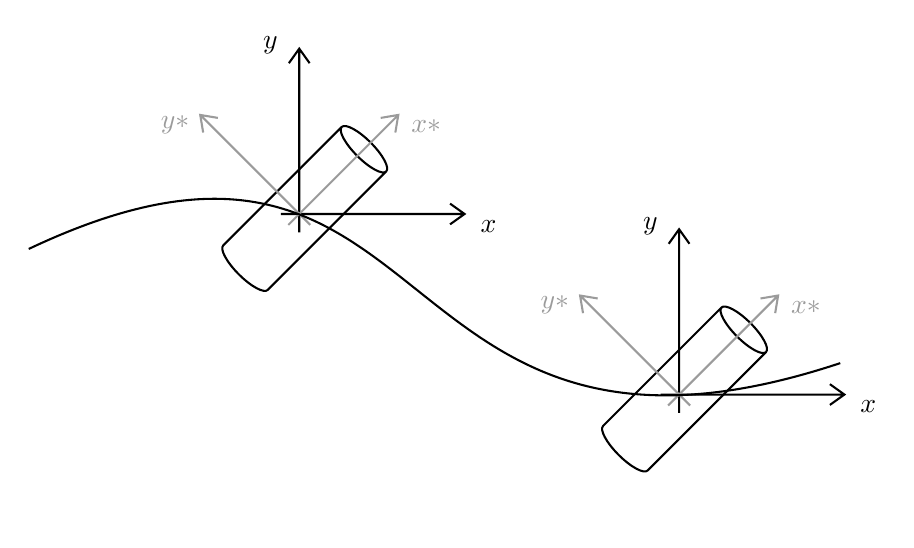
\begin{tikzpicture}[x=0.75pt,y=0.75pt,yscale=-1,xscale=1]
	%uncomment if require: \path (0,300); %set diagram left start at 0, and has height of 300

	%Shape: Can [id:dp6323252782775708] 
	\draw  [fill={rgb, 255:red, 255; green, 255; blue, 255 }  ,fill opacity=1 ] (295.74,99.68) -- (238.68,156.74) .. controls (236.91,158.52) and (230.66,155.16) .. (224.73,149.23) .. controls (218.81,143.3) and (215.44,137.06) .. (217.22,135.28) -- (274.28,78.22) .. controls (276.06,76.44) and (282.3,79.8) .. (288.23,85.73) .. controls (294.16,91.66) and (297.52,97.9) .. (295.74,99.68) .. controls (293.97,101.46) and (287.72,98.1) .. (281.79,92.17) .. controls (275.87,86.24) and (272.5,80) .. (274.28,78.22) ;
	%Shape: Axis 2D [id:dp7646233898089312] 
	\draw  (245,120.15) -- (333.5,120.15)(253.85,40.5) -- (253.85,129) (326.5,115.15) -- (333.5,120.15) -- (326.5,125.15) (248.85,47.5) -- (253.85,40.5) -- (258.85,47.5)  ;
	%Shape: Axis 2D [id:dp5228073483027118] 
	\draw [color={rgb, 255:red, 155; green, 155; blue, 155 }  ,draw opacity=1 ] (248.55,125.45) -- (301.56,72.44)(206.14,72.44) -- (259.15,125.45) (293.07,73.86) -- (301.56,72.44) -- (300.14,80.93) (207.56,80.93) -- (206.14,72.44) -- (214.63,73.86)  ;
	%Shape: Can [id:dp6975388475569626] 
	\draw  [fill={rgb, 255:red, 255; green, 255; blue, 255 }  ,fill opacity=1 ] (478.74,186.68) -- (421.68,243.74) .. controls (419.91,245.52) and (413.66,242.16) .. (407.73,236.23) .. controls (401.81,230.3) and (398.44,224.06) .. (400.22,222.28) -- (457.28,165.22) .. controls (459.06,163.44) and (465.3,166.8) .. (471.23,172.73) .. controls (477.16,178.66) and (480.52,184.9) .. (478.74,186.68) .. controls (476.97,188.46) and (470.72,185.1) .. (464.79,179.17) .. controls (458.87,173.24) and (455.5,167) .. (457.28,165.22) ;
	%Shape: Axis 2D [id:dp7028463504592724] 
	\draw  (428,207.15) -- (516.5,207.15)(436.85,127.5) -- (436.85,216) (509.5,202.15) -- (516.5,207.15) -- (509.5,212.15) (431.85,134.5) -- (436.85,127.5) -- (441.85,134.5)  ;
	%Shape: Axis 2D [id:dp5515393672066395] 
	\draw [color={rgb, 255:red, 155; green, 155; blue, 155 }  ,draw opacity=1 ] (431.55,212.45) -- (484.56,159.44)(389.14,159.44) -- (442.15,212.45) (476.07,160.86) -- (484.56,159.44) -- (483.14,167.93) (390.56,167.93) -- (389.14,159.44) -- (397.63,160.86)  ;
	%Curve Lines [id:da08058788370798475] 
	\draw    (123.5,137) .. controls (326.5,41) and (288.5,267) .. (514.5,192) ;

	% Text Node
	\draw (345,126) node    {$x$};
	% Text Node
	\draw (240,39) node    {$y$};
	% Text Node
	\draw (315,78) node  [color={rgb, 255:red, 155; green, 155; blue, 155 }  ,opacity=1 ]  {$x*$};
	% Text Node
	\draw (194,77) node  [color={rgb, 255:red, 155; green, 155; blue, 155 }  ,opacity=1 ]  {$y*$};
	% Text Node
	\draw (528,213) node    {$x$};
	% Text Node
	\draw (423,126) node    {$y$};
	% Text Node
	\draw (498,165) node  [color={rgb, 255:red, 155; green, 155; blue, 155 }  ,opacity=1 ]  {$x*$};
	% Text Node
	\draw (377,164) node  [color={rgb, 255:red, 155; green, 155; blue, 155 }  ,opacity=1 ]  {$y*$};

	\end{tikzpicture}
\end{figure}
\FloatBarrier
Studiare le equazioni cardinali della dinamica permette di ricavare il moto del sistema. Si impone anche la condizione che il corpo non ruoti.

\[
	\vec{R} = m\,\vec{a}_{cm} 	\quad \vec{M} = 0
\]

Il problema potrebbe essere studiato anche da un punto di vista energetico dicendo che il lavoro di tutte le forze è uguale alla variazione di energia cinetica subita dal corpo rigido.

\[
	\mathcal{L} = \Delta E_K \quad E_K = \sum_i \frac{1}{2}  m_i v_i^2  = \frac{1}{2} \sum_i m_i v_{cm}^2  = \frac{1}{2} M\,v_{cm}^2
\]

in caso di traslazione l'energia cinetica del corpo rigido è uguale all'energia cinetica del solo centro di massa. Si può sostituire questa relazione a una delle due equazioni cardinali della dinamica. Tale risultato non contraddice il teorema di K\"onig perché se si considera un osservatore sul centro di massa, esso non vede le parti intorno a sé che si muovono.

\paragraph{Esempio} Si consideri lo stesso problema affrontato in precedenza. Si ha lo stesso parallelepipedo che deve essere trascinato su un piano scabro. La velocità può essere una funzione del tempo, il corpo in generale non si muove di moto uniforme. Si utilizzano le leggi della dinamica e, definito un asse orizzontale $x$, si avrà:

\begin{gather*}
	\underbrace{F_o\,H - R_n x}_{\vec{M}} = 0 \\
	F_o - \mu_d R_n = Ma_{cm} \implies \frac{F}{M} - \mu_d g = a_{cm}
\end{gather*}

Si sceglie come polo $O$ il punto sulla verticale passante per il centro di massa, sul piano d'appoggio. Le uniche due forze che generano momento saranno $\vec{F}_o$ e $\vec{R}_n$.

\subsection{Rotazione del corpo rigido}

In tale tipo di moto, le varie parti del corpo rigido si muovono seguendo come traiettoria delle circonferenze che hanno centro sull'asse di rotazione e che giacciono su un piano ortogonale ad esso.

\begin{figure}[htpb]
	\centering

	\tikzset{every picture/.style={line width=0.75pt}} %set default line width to 0.75pt        

	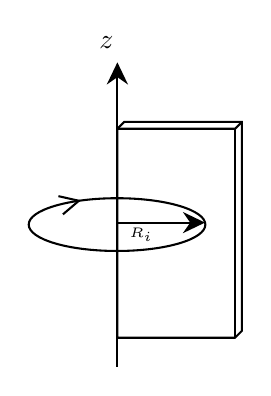
\begin{tikzpicture}[x=0.75pt,y=0.75pt,yscale=-1,xscale=1]
	%uncomment if require: \path (0,300); %set diagram left start at 0, and has height of 300

	%Straight Lines [id:da50179012944499] 
	\draw    (240.5,201.67) -- (240.5,58) ;
	\draw [shift={(240.5,55)}, rotate = 450] [fill={rgb, 255:red, 0; green, 0; blue, 0 }  ][line width=0.08]  [draw opacity=0] (10.72,-5.15) -- (0,0) -- (10.72,5.15) -- (7.12,0) -- cycle    ;
	%Shape: Cube [id:dp757166379594971] 
	\draw   (240.5,87) -- (243.83,83.67) -- (300.5,83.67) -- (300.5,184.33) -- (297.17,187.67) -- (240.5,187.67) -- cycle ; \draw   (300.5,83.67) -- (297.17,87) -- (240.5,87) ; \draw   (297.17,87) -- (297.17,187.67) ;
	%Shape: Ellipse [id:dp23280864685067515] 
	\draw   (197.78,133.16) .. controls (197.78,126.14) and (216.83,120.45) .. (240.33,120.45) .. controls (263.84,120.45) and (282.89,126.14) .. (282.89,133.16) .. controls (282.89,140.18) and (263.84,145.87) .. (240.33,145.87) .. controls (216.83,145.87) and (197.78,140.18) .. (197.78,133.16) -- cycle ;
	\draw   (212.1,119.46) -- (221.95,121.69) -- (214.26,128.23) ;
	%Straight Lines [id:da3343461623953874] 
	\draw    (240.33,132.2) -- (279.72,132.2) ;
	\draw [shift={(282.72,132.2)}, rotate = 180] [fill={rgb, 255:red, 0; green, 0; blue, 0 }  ][line width=0.08]  [draw opacity=0] (10.72,-5.15) -- (0,0) -- (10.72,5.15) -- (7.12,0) -- cycle    ;

	% Text Node
	\draw (235.2,45.6) node    {$z$};
	% Text Node
	\draw (252,138) node  [font=\tiny]  {$R_{i}$};

	\end{tikzpicture}
\end{figure}
\FloatBarrier
I vari punti del corpo avranno velocità che è tangente alla circonferenza. Essa in generale non è sempre uguale perché i punti più all'esterno devono compiere in ugual tempo una circonferenza maggiore. La quantità che si mantiene uguale è $\omega$. $\vec{\omega}$ e $\vec{R}$ sono ortogonali tra di loro.

\[
	\vec{v}_i =\vec{\omega} \times \vec{R}_i \qquad v_i=\omega \,R_i
\]

Questa condizione è quella che caratterizza la rotazione del corpo rigido. Il problema si sposta nello studiare nel tempo come variano $\omega$ e $\alpha$, parametri univoci per ogni punto del corpo.

\paragraph{Rotazioni rigide attorno ad un asse fisso in un sistema di riferimento inerziale} Si studia il moto di rotazione di un corpo rigido intorno a un asse fisso $z$. La caratteristica fondamentale nel moto di rotazione del corpo rigido intorno ad un asse è che fondamentalmente tutti i punti di esso si vanno a muovere su delle circonferenze, poste su piani paralleli tra di loro, quindi complanari. I vari punti del corpo possiedono velocità diverse tra loro, ma hanno stessa velocità angolare. Quindi, i punti più lontani dall'asse dovranno avere velocità maggiore per poter percorrere nello stesso tempo una circonferenza di raggio maggiore. Il vettore velocità angolare, parallelo all'asse $z$, diventa la caratteristica cinematica che bisogna calcolare a partire dalla conoscenza delle forze, e in particolare del momento delle forze, applicate al corpo rigido. Si utilizzeranno le equazioni cardinali della dinamica.

\begin{gather*}
	v_i = \omega \, R_i \quad \vec{\omega}_i = \vec{\omega} \;\; \forall i \qquad \vec{\omega} \parallel \vec{u}_z \\
	\vec{M}_{tot}^{(o)} = \frac{ d\vec{L}_{tot}^{(o)}  }{dt} - \vec{v}_o\times M\vec{v}_{cm}
\end{gather*}

Il polo lo si prende sull'asse quindi la sua velocità vale zero: si può eliminare il secondo termine. Ora, bisogna trovare il modo per esprimere in maniera più semplice il momento angolare complessivo del sistema di punti. Si calcola $\vec{L}_\text{tot}$:

\[
	\vec{L}_{tot}^{(o)} = \sum_i^n \vec{r}\,^{(o)}_i \times m_i\vec{v}_i
\]

Il raggio vettore $\vec{r}_i$ che congiunge il polo $o$ alla massa $i$-esima è quello in figura. Contemporaneamente si può rilevare la direzione della velocità del corpo, se esso sta ruotando intorno all'asse $z$. Ad esempio,
nel punto $A$ la velocità avrà direzione entrante al piano del foglio. Si osserva che il raggio vettore può essere visto come la somma di due contributi. In particolare modo esso è dato dalla somma vettoriale fra $\vec{R}_i$ e un secondo vettore $\vec{z}_i$ e che identifica la quota a cui si trova la massa rispetto al polo:

\[
	\vec{r}_i = \vec{z}_i +\vec{R}_i
\]

Sostituendo si ha:

\[
	\vec{L}_{tot}^{(o)} = \sum_i \left( \vec{z}_i+\vec{R}_i\right) \times m_i\vec{v}_i
\]

Applicando la proprietà distributiva:

\[
	\sum_i \left( \vec{z}_i\times m_i\vec{v}_i    \right) + \sum_i \left( \vec{R}_i\times m_i\vec{v}_i \right)
\]

Nascono due termini che sono entrambi momenti angolari.

\begin{itemize}
	\item Primo termine. $\vec{z}_i$ è diretto verso l'alto, $\vec{v}_i$ è sempre entrante nel piano del foglio. Il risultato del prodotto vettoriale è un vettore che giace sempre nel piano ortogonale all'asse $z$ e che è sempre diretto con verso centripeto a tale asse. Tale termine nella sommatoria prende il nome di \emph{momento angolare ortogonale $i$-esimo}, o anche \emph{momento angolare radiale}, perché è parallelo al raggio.
	\item Secondo termine. $\norm{\vec{R}_i}$ è la distanza assiale. $\vec{v}_i$ nel disegno è entrante al piano del foglio. Il prodotto vettoriale è quindi un vettore parallelo all'asse $z$. Il termine dentro la sommatoria lo si chiama quindi \emph{momento angolare assiale $i$-esimo}.
\end{itemize}

Il generico punto $i$ sarà dotato di un momento angolare ortogonale e uno assiale. Si considerino le masse $m_i$ ed $m_j$ come in figura.

\begin{figure}[htpb]
	\centering

	\tikzset{every picture/.style={line width=0.75pt}} %set default line width to 0.75pt        

	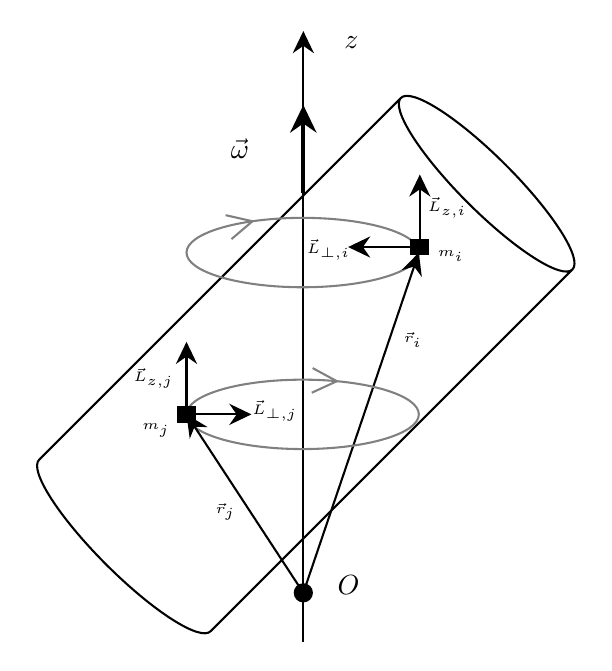
\begin{tikzpicture}[x=0.75pt,y=0.75pt,yscale=-1,xscale=1]
	%uncomment if require: \path (0,376); %set diagram left start at 0, and has height of 376

	%Straight Lines [id:da5195660360442784] 
	\draw    (255.74,330.5) -- (255.74,39.34) ;
	\draw [shift={(255.74,36.34)}, rotate = 450] [fill={rgb, 255:red, 0; green, 0; blue, 0 }  ][line width=0.08]  [draw opacity=0] (10.72,-5.15) -- (0,0) -- (10.72,5.15) -- (7.12,0) -- cycle    ;
	%Shape: Can [id:dp8455999264544007] 
	\draw   (385.39,151.22) -- (211.11,325.49) .. controls (206.08,330.52) and (183.5,316.1) .. (160.67,293.27) .. controls (137.85,270.45) and (123.43,247.86) .. (128.46,242.83) -- (302.73,68.56) .. controls (307.76,63.53) and (330.35,77.95) .. (353.17,100.77) .. controls (376,123.6) and (390.42,146.18) .. (385.39,151.22) .. controls (380.35,156.25) and (357.77,141.83) .. (334.94,119) .. controls (312.12,96.18) and (297.7,73.59) .. (302.73,68.56) ;
	%Shape: Ellipse [id:dp9697851711980743] 
	\draw  [color={rgb, 255:red, 128; green, 128; blue, 128 }  ,draw opacity=1 ] (199.45,143.06) .. controls (199.45,133.83) and (224.51,126.34) .. (255.42,126.34) .. controls (286.33,126.34) and (311.39,133.83) .. (311.39,143.06) .. controls (311.39,152.3) and (286.33,159.78) .. (255.42,159.78) .. controls (224.51,159.78) and (199.45,152.3) .. (199.45,143.06) -- cycle ;
	\draw  [color={rgb, 255:red, 128; green, 128; blue, 128 }  ,draw opacity=1 ] (218.29,125.05) -- (231.24,127.98) -- (221.12,136.58) ;
	%Straight Lines [id:da36834618504300853] 
	\draw [line width=1.5]    (255.74,114.56) -- (255.74,75.98) ;
	\draw [shift={(255.74,71.98)}, rotate = 450] [fill={rgb, 255:red, 0; green, 0; blue, 0 }  ][line width=0.08]  [draw opacity=0] (13.4,-6.43) -- (0,0) -- (13.4,6.44) -- (8.9,0) -- cycle    ;
	%Straight Lines [id:da9652713306447409] 
	\draw [line width=0.75]    (255.74,307) -- (310.43,145.9) ;
	\draw [shift={(311.39,143.06)}, rotate = 468.75] [fill={rgb, 255:red, 0; green, 0; blue, 0 }  ][line width=0.08]  [draw opacity=0] (10.72,-5.15) -- (0,0) -- (10.72,5.15) -- (7.12,0) -- cycle    ;
	%Shape: Ellipse [id:dp3060968998104503] 
	\draw  [fill={rgb, 255:red, 0; green, 0; blue, 0 }  ,fill opacity=1 ] (251.62,307) .. controls (251.62,304.73) and (253.46,302.89) .. (255.74,302.89) .. controls (258.01,302.89) and (259.85,304.73) .. (259.85,307) .. controls (259.85,309.28) and (258.01,311.12) .. (255.74,311.12) .. controls (253.46,311.12) and (251.62,309.28) .. (251.62,307) -- cycle ;
	%Shape: Rectangle [id:dp5101136247809177] 
	\draw  [fill={rgb, 255:red, 0; green, 0; blue, 0 }  ,fill opacity=1 ] (307.86,136.93) -- (315.87,136.93) -- (315.87,143.87) -- (307.86,143.87) -- cycle ;
	%Straight Lines [id:da6918942322173436] 
	\draw [line width=0.75]    (311.87,140.4) -- (311.87,108.45) ;
	\draw [shift={(311.87,105.45)}, rotate = 450] [fill={rgb, 255:red, 0; green, 0; blue, 0 }  ][line width=0.08]  [draw opacity=0] (10.72,-5.15) -- (0,0) -- (10.72,5.15) -- (7.12,0) -- cycle    ;
	%Straight Lines [id:da48439494498668956] 
	\draw [line width=0.75]    (311.87,140.4) -- (280.32,140.4) ;
	\draw [shift={(277.32,140.4)}, rotate = 360] [fill={rgb, 255:red, 0; green, 0; blue, 0 }  ][line width=0.08]  [draw opacity=0] (10.72,-5.15) -- (0,0) -- (10.72,5.15) -- (7.12,0) -- cycle    ;
	%Shape: Ellipse [id:dp7304179034589999] 
	\draw  [color={rgb, 255:red, 128; green, 128; blue, 128 }  ,draw opacity=1 ] (199.45,221.02) .. controls (199.45,211.79) and (224.51,204.3) .. (255.42,204.3) .. controls (286.33,204.3) and (311.39,211.79) .. (311.39,221.02) .. controls (311.39,230.25) and (286.33,237.74) .. (255.42,237.74) .. controls (224.51,237.74) and (199.45,230.25) .. (199.45,221.02) -- cycle ;
	\draw  [color={rgb, 255:red, 128; green, 128; blue, 128 }  ,draw opacity=1 ] (260.22,198.72) -- (271.89,205.05) -- (259.82,210.59) ;
	%Straight Lines [id:da26215718910091446] 
	\draw [line width=0.75]    (255.74,307) -- (201.1,223.53) ;
	\draw [shift={(199.45,221.02)}, rotate = 416.78999999999996] [fill={rgb, 255:red, 0; green, 0; blue, 0 }  ][line width=0.08]  [draw opacity=0] (10.72,-5.15) -- (0,0) -- (10.72,5.15) -- (7.12,0) -- cycle    ;
	%Shape: Rectangle [id:dp4523941492080834] 
	\draw  [fill={rgb, 255:red, 0; green, 0; blue, 0 }  ,fill opacity=1 ] (195.45,217.55) -- (203.46,217.55) -- (203.46,224.49) -- (195.45,224.49) -- cycle ;
	%Straight Lines [id:da3397567748160464] 
	\draw [line width=0.75]    (199.45,221.02) -- (199.45,189.07) ;
	\draw [shift={(199.45,186.07)}, rotate = 450] [fill={rgb, 255:red, 0; green, 0; blue, 0 }  ][line width=0.08]  [draw opacity=0] (10.72,-5.15) -- (0,0) -- (10.72,5.15) -- (7.12,0) -- cycle    ;
	%Straight Lines [id:da002150672325501146] 
	\draw [line width=0.75]    (199.45,221.02) -- (227.73,221.02) ;
	\draw [shift={(230.73,221.02)}, rotate = 180] [fill={rgb, 255:red, 0; green, 0; blue, 0 }  ][line width=0.08]  [draw opacity=0] (10.72,-5.15) -- (0,0) -- (10.72,5.15) -- (7.12,0) -- cycle    ;

	% Text Node
	\draw (278.86,42.03) node    {$z$};
	% Text Node
	\draw (225.22,93.01) node    {$\vec{\omega }$};
	% Text Node
	\draw (277.53,303.02) node    {$O$};
	% Text Node
	\draw (308.54,185.12) node  [font=\tiny]  {$\vec{r}_{i}$};
	% Text Node
	\draw (325.02,121.71) node  [font=\tiny]  {$\vec{L}_{z,i}$};
	% Text Node
	\draw (267.84,141.85) node  [font=\tiny]  {$\vec{L}_{\bot ,i}$};
	% Text Node
	\draw (326.74,144.84) node  [font=\tiny]  {$m_{i}$};
	% Text Node
	\draw (218.24,267.9) node  [font=\tiny]  {$\vec{r}_{j}$};
	% Text Node
	\draw (183.6,203.67) node  [font=\tiny]  {$\vec{L}_{z,j}$};
	% Text Node
	\draw (242.02,219.47) node  [font=\tiny]  {$\vec{L}_{\bot ,j}$};
	% Text Node
	\draw (184.81,228.8) node  [font=\tiny]  {$m_{j}$};

	\end{tikzpicture}
\end{figure}
\FloatBarrier
Si osservi come cambiano le direzioni dei momenti. La velocità della massa $m_j$ sarà uscente dal piano del foglio. Il momento angolare assiale è concorde a quello precedente della massa $i$-esima. Anche il suo momento ortogonale punta verso l'asse. Se si considerano tutte le masse infinitesime, si avrà un momento angolare assiale dato dalla somma di tanti contributi tutti concordi fra di loro in direzione e verso. Quindi si dovrà semplicemente sommarli scalarmente, ottenendo $\vec{L}_z$, il \textbf{momento angolare assiale}. Il termine che nasce invece sommando tutti i momenti angolari ortogonali $i$-esimi, ossia il \textbf{momento angolare radiale}, lo si indica invece con $\vec{L}_\perp$. Il momento angolare totale rispetto al polo $O$ sarà dato dalla somma di $\vec{L}_z$ e $\vec{L}_\perp$.

\[
	\boxed{\vec{L}_{tot}^{(o)} = \vec{L}_z + \vec{L}_{\bot}}
\]

\paragraph{Momento angolare assiale}

\begin{itemize}
	\item I vettori sono tutti paralleli tra loro, diretti come $\vec{u}_z$ e concordi, il prodotto vettoriale sarà dato dal prodotto fra i moduli
	\[
		\vec{L}_z = \sum_i R_i m_i v_i \vec{u}_z
	\]
	\item La velocità scalare che possiede ogni punto materiale è legata alla velocità angolare, si può sostituire $v_i$ con $\omega R_i$
	\[
		\vec{L}_z = \sum_i \left(R_i m_i\omega R_i \right) \vec{u}_z
	\]
	\item A questo punto si porta fuori $\omega$ dalla sommatoria perché è in comune a tutti gli angoli.
	\[
		\vec{L}_z = \underbrace{\left( \sum_i m_i R_i^2 \right) \cdot \omega \vec{u}_z}_{\vec{\omega} \parallel \vec{u}_z \implies \omega \cdot \vec{u}_z = \vec{\omega}} = \sum_i \left( m_i R_i^2  \right) \cdot \vec{\omega}
	\]
\end{itemize}

Il termine evidenziato dipende dalla geometria del corpo e in particolare da quanta è la sua massa e come questa è distribuita rispetto all'asse $z$. Si tratta di una quantità caratteristica del corpo esteso e prende il nome di \textbf{momento di inerzia del corpo} rispetto all'asse $z$. Viene indicato con la lettera $I$ ed è una quantità scalare. Va sottolineato sempre a pedice qual è l'asse $z$ rispetto a cui si sta indicando questa proprietà del corpo. Infatti, se si fa ruotare il corpo in un modo, attorno a un certo asse, si avrà un certo momento di inerzia. Tuttavia, se lo si fa ruotare in un altra maniera, attorno ad un asse diverso, anche il momento di inerzia sarà diverso. Esso dipende quindi anche dall'asse di rotazione.

\[
	\boxed{I_z = \sum_i^n m_i\,R_i^2} \qquad \text{Momento d'inerzia}
\]

\paragraph{Momento angolare radiale} Finora fondamentalmente è stato detto che, senza più suddividere il corpo in tante parti, esso è dotato di una componente del momento angolare totale diretto parallelamente all'asse $z$. È possibile dire lo stesso del momento angolare radiale? Ossia, si può andare a calcolare la somma vettoriale di tutti i momenti ortogonali $i$-esimi e far vedere che le varie componenti della somma hanno la stessa direzione, in modo tale da dare come risultato a loro volta un vettore avente ugual direzione? La risposta ovviamente è negativa, e ciò complica notevolmente il calcolo di tale termine. Infatti, i momenti radiali $i$-esimi sono vettori che puntano sempre verso l'asse di rotazione.

\begin{figure}[htpb]
	\centering

	\tikzset{every picture/.style={line width=0.75pt}} %set default line width to 0.75pt        

	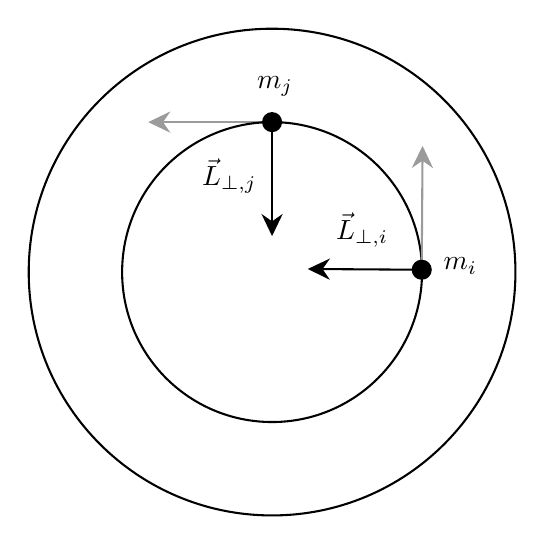
\begin{tikzpicture}[x=0.75pt,y=0.75pt,yscale=-1,xscale=1]
	%uncomment if require: \path (0,300); %set diagram left start at 0, and has height of 300

	%Straight Lines [id:da12459801471491572] 
	\draw [color={rgb, 255:red, 155; green, 155; blue, 155 }  ,draw opacity=1 ]   (287.25,90) -- (230.58,90) ;
	\draw [shift={(227.58,90)}, rotate = 360] [fill={rgb, 255:red, 155; green, 155; blue, 155 }  ,fill opacity=1 ][line width=0.08]  [draw opacity=0] (10.72,-5.15) -- (0,0) -- (10.72,5.15) -- (7.12,0) -- cycle    ;
	%Shape: Ellipse [id:dp23179179531682093] 
	\draw   (170,162.25) .. controls (170,97.49) and (222.49,45) .. (287.25,45) .. controls (352.01,45) and (404.5,97.49) .. (404.5,162.25) .. controls (404.5,227.01) and (352.01,279.5) .. (287.25,279.5) .. controls (222.49,279.5) and (170,227.01) .. (170,162.25) -- cycle ;
	%Shape: Ellipse [id:dp9965082237761831] 
	\draw   (215,162.25) .. controls (215,122.35) and (247.35,90) .. (287.25,90) .. controls (327.15,90) and (359.5,122.35) .. (359.5,162.25) .. controls (359.5,202.15) and (327.15,234.5) .. (287.25,234.5) .. controls (247.35,234.5) and (215,202.15) .. (215,162.25) -- cycle ;
	%Shape: Circle [id:dp055117462910539095] 
	\draw  [fill={rgb, 255:red, 0; green, 0; blue, 0 }  ,fill opacity=1 ] (282.92,90) .. controls (282.92,87.61) and (284.86,85.67) .. (287.25,85.67) .. controls (289.64,85.67) and (291.58,87.61) .. (291.58,90) .. controls (291.58,92.39) and (289.64,94.33) .. (287.25,94.33) .. controls (284.86,94.33) and (282.92,92.39) .. (282.92,90) -- cycle ;
	%Straight Lines [id:da041846034904831075] 
	\draw    (287.25,90) -- (287.25,141.92) ;
	\draw [shift={(287.25,144.92)}, rotate = 270] [fill={rgb, 255:red, 0; green, 0; blue, 0 }  ][line width=0.08]  [draw opacity=0] (10.72,-5.15) -- (0,0) -- (10.72,5.15) -- (7.12,0) -- cycle    ;
	%Straight Lines [id:da11385728118969496] 
	\draw [color={rgb, 255:red, 155; green, 155; blue, 155 }  ,draw opacity=1 ]   (359.35,161.13) -- (359.74,104.46) ;
	\draw [shift={(359.76,101.46)}, rotate = 450.39] [fill={rgb, 255:red, 155; green, 155; blue, 155 }  ,fill opacity=1 ][line width=0.08]  [draw opacity=0] (10.72,-5.15) -- (0,0) -- (10.72,5.15) -- (7.12,0) -- cycle    ;
	%Shape: Circle [id:dp8931699931661818] 
	\draw  [fill={rgb, 255:red, 0; green, 0; blue, 0 }  ,fill opacity=1 ] (359.38,156.8) .. controls (361.78,156.81) and (363.7,158.77) .. (363.69,161.16) .. controls (363.67,163.55) and (361.72,165.48) .. (359.32,165.46) .. controls (356.93,165.45) and (355,163.49) .. (355.02,161.1) .. controls (355.04,158.71) and (356.99,156.78) .. (359.38,156.8) -- cycle ;
	%Straight Lines [id:da7193380899952875] 
	\draw    (359.35,161.13) -- (307.44,160.78) ;
	\draw [shift={(304.44,160.76)}, rotate = 360.39] [fill={rgb, 255:red, 0; green, 0; blue, 0 }  ][line width=0.08]  [draw opacity=0] (10.72,-5.15) -- (0,0) -- (10.72,5.15) -- (7.12,0) -- cycle    ;

	% Text Node
	\draw (288.67,72.67) node    {$m_{j}$};
	% Text Node
	\draw (266.67,116) node    {$\vec{L}_{\bot ,j}$};
	% Text Node
	\draw (330.67,142) node    {$\vec{L}_{\bot ,i}$};
	% Text Node
	\draw (378,159.33) node    {$m_{i}$};

	\end{tikzpicture}
\end{figure}
\FloatBarrier
Si immagini che a fianco sia raffigurato il cilindro disegnato in precedenza, visto dall'alto. Il problema è che se bisogna sommare tutti i vettori della forma che si osserva a lato, essi non hanno stessa direzione e il calcolo è più complicato.

Otteniamo quindi che

\[
	\vec{L}_{\bot} = \sum_i z_i m_i v_i \vec{u}_{\bot,i} = \sum_i z_i m_i\omega R_i\vec{u}_{\bot,i} = \sum_i (z_i m_i R_i \vec{u}_{\bot,i})\omega
\]

Il calcolo è complesso, ma si può notare una cosa importante quando l'asse di rotazione è un asse di simmetria per il corpo, ed esso è omogeneo.

\begin{figure}[htpb]
	\centering

	\tikzset{every picture/.style={line width=0.75pt}} %set default line width to 0.75pt        

	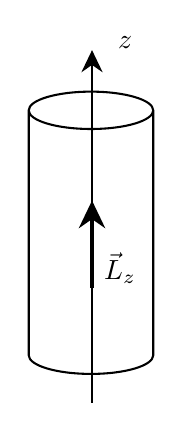
\begin{tikzpicture}[x=0.75pt,y=0.75pt,yscale=-1,xscale=1]
	%uncomment if require: \path (0,300); %set diagram left start at 0, and has height of 300

	%Straight Lines [id:da4575961066685954] 
	\draw    (263.5,252) -- (263.5,85) ;
	\draw [shift={(263.5,82)}, rotate = 450] [fill={rgb, 255:red, 0; green, 0; blue, 0 }  ][line width=0.08]  [draw opacity=0] (10.72,-5.15) -- (0,0) -- (10.72,5.15) -- (7.12,0) -- cycle    ;
	%Shape: Can [id:dp23997666541951923] 
	\draw   (293,111) -- (293,229) .. controls (293,233.97) and (279.57,238) .. (263,238) .. controls (246.43,238) and (233,233.97) .. (233,229) -- (233,111) .. controls (233,106.03) and (246.43,102) .. (263,102) .. controls (279.57,102) and (293,106.03) .. (293,111) .. controls (293,115.97) and (279.57,120) .. (263,120) .. controls (246.43,120) and (233,115.97) .. (233,111) ;
	%Straight Lines [id:da9486642752628265] 
	\draw [line width=1.5]    (263.5,196.5) -- (263.5,158.5) ;
	\draw [shift={(263.5,154.5)}, rotate = 450] [fill={rgb, 255:red, 0; green, 0; blue, 0 }  ][line width=0.08]  [draw opacity=0] (13.4,-6.43) -- (0,0) -- (13.4,6.44) -- (8.9,0) -- cycle    ;

	% Text Node
	\draw (279.5,78.5) node    {$z$};
	% Text Node
	\draw (277,187) node    {$\vec{L}_{z}$};

	\end{tikzpicture}
\end{figure}
\FloatBarrier
Infatti, considerando soltanto la componente $\vec{L}_\perp$, presa la massa $i$-esima che avrà un certo momento ortogonale $i$-esimo, esisterà sempre una massa $m_j$ posta in posizione simmetrica alla massa $m_i$ tale per cui nascerà la componente radiale del momento angolare $j$-esima che andrà annullare quella $i$-esima. La massa $j$ infatti sarà alla stessa quota di $i$ (stesso $z_i$), avrà raggio $R_i$ e il suo momento $\vec{L}_j$ sarà uguale e opposto a $\vec{L}_i$. Allora Il momento angolare totale è formato soltanto dalla componente assiale.

Se $\vec{L}_\perp$ è diverso da zero, si può dimostrare che fondamentalmente è una componente che punterà sempre verso l'asse facendo la somma vettoriale totale. $\vec{L}_\text{tot}$ sarà allora diretto come in figura.

\begin{figure}[htpb]
	\centering

	\tikzset{every picture/.style={line width=0.75pt}} %set default line width to 0.75pt        

	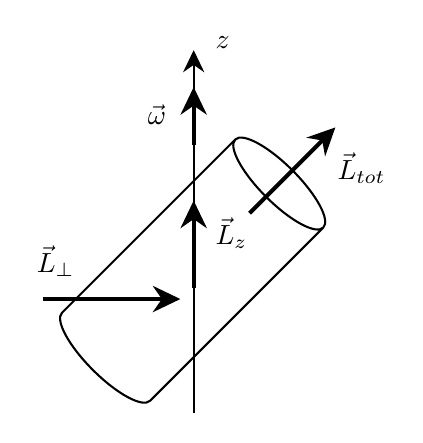
\begin{tikzpicture}[x=0.75pt,y=0.75pt,yscale=-1,xscale=1]
	%uncomment if require: \path (0,300); %set diagram left start at 0, and has height of 300

	%Straight Lines [id:da3478243083512724] 
	\draw    (263.5,239) -- (263.5,67) ;
	\draw [shift={(263.5,64)}, rotate = 450] [fill={rgb, 255:red, 0; green, 0; blue, 0 }  ][line width=0.08]  [draw opacity=0] (10.72,-5.15) -- (0,0) -- (10.72,5.15) -- (7.12,0) -- cycle    ;
	%Shape: Can [id:dp3112940153689916] 
	\draw   (325.93,149.49) -- (242.49,232.93) .. controls (238.98,236.45) and (226.63,229.8) .. (214.92,218.08) .. controls (203.2,206.37) and (196.55,194.02) .. (200.07,190.51) -- (283.51,107.07) .. controls (287.02,103.55) and (299.37,110.2) .. (311.08,121.92) .. controls (322.8,133.63) and (329.45,145.98) .. (325.93,149.49) .. controls (322.42,153.01) and (310.07,146.36) .. (298.36,134.64) .. controls (286.64,122.93) and (279.99,110.58) .. (283.51,107.07) ;
	%Straight Lines [id:da11426354012586315] 
	\draw [line width=1.5]    (263.5,178.5) -- (263.5,140.5) ;
	\draw [shift={(263.5,136.5)}, rotate = 450] [fill={rgb, 255:red, 0; green, 0; blue, 0 }  ][line width=0.08]  [draw opacity=0] (13.4,-6.43) -- (0,0) -- (13.4,6.44) -- (8.9,0) -- cycle    ;
	%Straight Lines [id:da11117414316202523] 
	\draw [line width=1.5]    (290.43,142.57) -- (328.91,104.09) ;
	\draw [shift={(331.74,101.26)}, rotate = 495] [fill={rgb, 255:red, 0; green, 0; blue, 0 }  ][line width=0.08]  [draw opacity=0] (13.4,-6.43) -- (0,0) -- (13.4,6.44) -- (8.9,0) -- cycle    ;
	%Straight Lines [id:da966548557557317] 
	\draw [line width=1.5]    (190.67,183.93) -- (253.07,183.93) ;
	\draw [shift={(257.07,183.93)}, rotate = 180] [fill={rgb, 255:red, 0; green, 0; blue, 0 }  ][line width=0.08]  [draw opacity=0] (13.4,-6.43) -- (0,0) -- (13.4,6.44) -- (8.9,0) -- cycle    ;
	%Straight Lines [id:da2931254655420723] 
	\draw [line width=1.5]    (263.5,109.67) -- (263.5,85.83) ;
	\draw [shift={(263.5,81.83)}, rotate = 450] [fill={rgb, 255:red, 0; green, 0; blue, 0 }  ][line width=0.08]  [draw opacity=0] (13.4,-6.43) -- (0,0) -- (13.4,6.44) -- (8.9,0) -- cycle    ;

	% Text Node
	\draw (277.5,60.5) node    {$z$};
	% Text Node
	\draw (281.67,152) node    {$\vec{L}_{z}$};
	% Text Node
	\draw (344.33,121) node    {$\vec{L}_{\text{tot}}$};
	% Text Node
	\draw (197,165.67) node    {$\vec{L}_{\bot }$};
	% Text Node
	\draw (245.83,95.17) node    {$\vec{\omega }$};

	\end{tikzpicture}
\end{figure}
\FloatBarrier
In generale, il momento angolare complessivo del corpo non è costante, ma ruota, si muove durante il moto. L'informazione data dal momento angolare totale non è utile per studiare come varia nel tempo la velocità angolare ma lo è solo per capire l'effetto delle forze di vincolo che permettono al corpo di ruotare rimanendo vincolato all'asse.

Concentrandosi sul momento angolare assiale in particolare, a questo punto bisogna collegare questa proprietà cinematica del corpo all'effetto dinamico delle forze, con la seconda equazione cardinale della dinamica. Si considereranno soltanto i momenti delle forze assiali, cioè quelle che danno luogo a un momento parallelo all'asse $z$, tali per cui vale la seconda equazione cardinale della dinamica. Si deriva di tale quantità.

\[
	\vec{M}^{(o)}_z = \frac{d\vec{L}_z }{dt} = \frac{d(I_z\vec{\omega}) }{dt} = I_z \vec{\alpha}
\]

Derivare è semplice perché $I_z$ non varia mentre il corpo si muove, perciò si può portarlo fuori dalla derivata. Rimane la derivata del vettore velocità angolare nel tempo, che è pari al vettore accelerazione angolare. Questa allora diventa la relazione della dinamica. Si può quindi calcolare i momenti delle forze diretti lungo l'asse $z$ e a questo punto si sarà in grado di ricavare qual è l'accelerazione angolare del corpo. Fondamentalmente è l'equivalente di utilizzare la seconda legge della dinamica per un punto materiale.

\[
	\boxed{\vec{M}_z = I_z\vec{\alpha}} \qquad \text{Legge fondamentale della dinamica}
\]

\begin{table}[H]
		\centering
		\begin{tabular}{c|c}
			Punto materiale & Corpo rigido in rotazione \\
			\hline
			$m$ & $I_z$ \\
			$\vec{p}$ & $\vec{L}$ \\
			$\vec{F} = \frac{d\vec{p} }{dt} = m\vec{a}$ & $\vec{M}^{(o)} = \frac{d\vec{L} }{dt}$ \\
			$\vec{F}_t = m\vec{a}_t$ & $\vec{M}_z=I_z\vec{\alpha}$ \\
			$\vec{F}_n = m\vec{a}_n$ & $\vec{M}_{\bot} = \frac{d\vec{L}_{\bot} }{dt}$
		\end{tabular}
	\end{table}
È utile fare un'analogia fra le proprietà introdotte per studiare il moto del punto materiale e quelle per il moto del corpo rigido in rotazione.

\begin{table}[H]
	\centering
	\begin{tabular}{|p{6.5cm}|p{6.5cm}|}
		\hline
		Punto materiale & Corpo rigido in rotazione \\
		\hline
		Il punto materiale lo si caratterizza con la \emph{massa inerziale}. Essa rappresenta l'inerzia del sistema, ossia la fatica che fa il corpo a cambiare il suo stato di moto rettilineo uniforme. & Ciò che caratterizza la fatica del corpo a essere messo in rotazione o, se si muove di moto uniforme, a far variare la velocità di rotazione, è il \emph{momento di inerzia}. Non basta solo la massa, ma conta come essa è distribuita intorno all'asse $x$. Dipende dalla forma del corpo e da come essa è posta rispetto all'asse $z$. \\
		\hline
		La \emph{quantità di moto} è l'inerzia di un corpo per la sua velocità. & La proprietà cinematica fondamentale di un corpo rigido in rotazione è il \emph{momento angolare}.\\
		\hline
		La \emph{seconda legge della dinamica} dice che la risultante delle forze provoca una variazione nel tempo della quantità di moto. & La variazione di $\vec{L}$ nel tempo è data dalla \emph{seconda equazione cardinale della dinamica}. Bisogna applicare una forza con momento tale da far variare il momento angolare, per far ruotare il corpo.\\
		\hline
		L'effetto delle forze che agiscono in direzione parallela alla traiettoria è diverso da quelle che agiscono in direzione tangente alla traiettoria. Le \emph{forze tangenziali} provocano un accelerazione tangente, fanno variare il modulo della velocità. & I momenti delle forze hanno effetti diversi a seconda di come sono diretti, in particolare i \emph{momenti assiali} delle forze sono quelli che hanno l'effetto di far variare il modulo della velocità angolare. \\
		\hline
		Le \emph{forze centripete} non fanno variare il modulo della velocità, ma ne fanno variare la direzione, permettono al corpo di percorrere una traiettoria curva. & Quelle forze che danno luogo a un \emph{momento ortogonale} all'asse $z$ provocano la variazione del momento angolare ortogonale nel tempo. Infatti, il momento angolare totale non è costante in direzione ma cambia.\\
		\hline
	\end{tabular}
\end{table}

Si vede ora come si calcola il momento di inerzia di un corpo.  Dato un corpo di forma estesa e definito un asse $z$ intorno a cui lo si vede ruotare, il momento di inerzia è definito come la somma di tutte le masse $i$-esime per il quadrato della distanza scalare fra la massa $i$-esima e l'asse $z$.

\[
	\sum_i m_i R_i^2  = I_z
\]

Questa è la forma che si userebbe se il corpo fosse una composizione discreta di masse. Se invece è un continuo, bisogna fare la somma continua fra tutte le masse infinitesime $dm$ per il quadrato della loro distanza. Questa somma continua la si estende a tutto il volume del corpo. Si avrà:

\[
	I_z = \sum_i m_i R_i^2  = \int_{\text{volume} }dm\,R^2 = \left\{ \begin{array}{l}
	 	\int_{\text{volume}} \rho R^2 dV \\
		\int_{\text{superficie}} \sigma R^2 dS \\
		\int_{\text{linea}} \lambda R^2 dl
	\end{array} \right.
\]

Dimensionalmente, il momento di inerzia è una massa per una distanza al quadrato. Per corpi di forme note o standard, esistono delle tabelle che riportano il momento di inerzia di corpi di forme standard per possibili assi $z$. Richiamiamo il momento di inerzia per alcuni di questi corpi.

\paragraph{Momento di inerzia di un anello} Si immagini di avere un anello di raggio $R$ e massa $M$.

\begin{figure}[htpb]
	\centering

	\tikzset{every picture/.style={line width=0.75pt}} %set default line width to 0.75pt        

	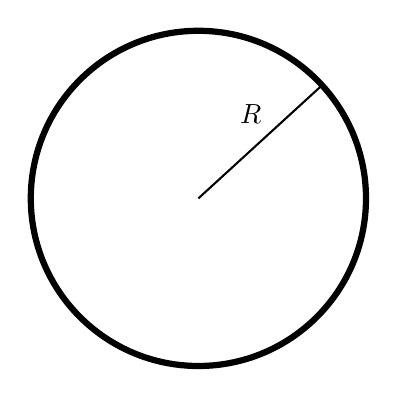
\begin{tikzpicture}[x=0.75pt,y=0.75pt,yscale=-1,xscale=1]
	%uncomment if require: \path (0,300); %set diagram left start at 0, and has height of 300

	%Shape: Circle [id:dp5232216239703855] 
	\draw  [line width=2.25]  (228,151.75) .. controls (228,107.15) and (264.15,71) .. (308.75,71) .. controls (353.35,71) and (389.5,107.15) .. (389.5,151.75) .. controls (389.5,196.35) and (353.35,232.5) .. (308.75,232.5) .. controls (264.15,232.5) and (228,196.35) .. (228,151.75) -- cycle ;
	%Straight Lines [id:da03854700022051927] 
	\draw    (308.75,151.75) -- (367.5,98) ;

	% Text Node
	\draw (334,111) node    {$R$};

	\end{tikzpicture}
\end{figure}
\FloatBarrier
Essa è distribuita solo sulla circonferenza. Bisogna capire qual è il suo momento di inerzia rispetto all'asse ortogonale al piano del foglio e passante per il centro dell'anello.

\[
	I_z = \int_{\text{linea}} dm\,R^2 = R^2 \int_{\text{linea}}dm = MR^2
\]

\paragraph{Momento di inerzia di un disco} Si ha un disco di massa $M$ e raggio $R$. Il momento di inerzia è, presa una massa infinitesima posta sul disco:

\[
	I_z = \int dm\,r^2
\]

Non si ha più $R$, perché in generale la distanza di ogni punto dal centro è diversa. Ogni punto dell'anello è alla stessa distanza dall'asse di rotazione.

\begin{figure}[htpb]
	\centering

	\tikzset{every picture/.style={line width=0.75pt}} %set default line width to 0.75pt        

	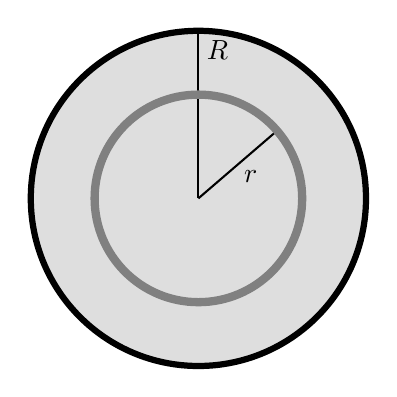
\begin{tikzpicture}[x=0.75pt,y=0.75pt,yscale=-1,xscale=1]
	%uncomment if require: \path (0,300); %set diagram left start at 0, and has height of 300

	%Shape: Circle [id:dp42752566168779715] 
	\draw  [color={rgb, 255:red, 0; green, 0; blue, 0 }  ,draw opacity=1 ][fill={rgb, 255:red, 222; green, 222; blue, 222 }  ,fill opacity=1 ][line width=2.25]  (228,151.75) .. controls (228,107.15) and (264.15,71) .. (308.75,71) .. controls (353.35,71) and (389.5,107.15) .. (389.5,151.75) .. controls (389.5,196.35) and (353.35,232.5) .. (308.75,232.5) .. controls (264.15,232.5) and (228,196.35) .. (228,151.75) -- cycle ;
	%Straight Lines [id:da7503358431498248] 
	\draw    (308.75,151.75) -- (308.75,71) ;
	%Straight Lines [id:da6185009717920751] 
	\draw    (308.75,151.75) -- (346.25,119.5) ;
	%Shape: Circle [id:dp4717670858472307] 
	\draw  [color={rgb, 255:red, 128; green, 128; blue, 128 }  ,draw opacity=1 ][line width=3]  (258.75,151.75) .. controls (258.75,124.14) and (281.14,101.75) .. (308.75,101.75) .. controls (336.36,101.75) and (358.75,124.14) .. (358.75,151.75) .. controls (358.75,179.36) and (336.36,201.75) .. (308.75,201.75) .. controls (281.14,201.75) and (258.75,179.36) .. (258.75,151.75) -- cycle ;

	% Text Node
	\draw (318,80.5) node    {$R$};
	% Text Node
	\draw (334,141) node    {$r$};

	\end{tikzpicture}
\end{figure}
\FloatBarrier
È necessario in questo caso risolvere un integrale di superficie, quindi doppio. Si può quindi ragionare come segue. Si pensa il disco come costituito da tante corone circolari (anelli di spessore infinitesimo) di raggio $r$ a cui è associato il momento di inerzia:

\[
	I_\text{z, corona}=M_\text{corona}r^2
\]

La massa su una corona circolare è data da:

\[
	\frac{\text{Area}_\text{corona}}{\text{Area}_\text{tot}}\, M=\frac{2\pi r\,dr}{\pi R^2} M
\]

Quindi:

\[
	I_\text{z, corona}=\frac{2 r\,dr}{R^2}M r^2
\]

Il momento di inerzia del disco, essendo una quantità additiva, è dato dalla somma dei momenti di inerzia associati alle singole corone, i cui raggi variano con continuità da 0 a $R$:

\[
	i_z=\int_0^R \frac{2}{R^2}r^3M\,dr=\frac{2}{R^2}M\biggl[\frac{r^4}{4} \biggr]_0^R=\frac{1}{2}MR^2
\]

La cosa interessante di questo risultato è che a pari massa e a pari raggio un disco presenta un momento di inerzia inferiore di un anello. Questo vuol dire che a pari forza applicata, o a pari momento di forze applicate, il disco accelererà con accelerazione maggiore dell'anello. Questo lo si può dimostrare. Se si prende un piano inclinato e ci si fa scendere un anello di massa $m$ e raggio $R$ e poi un disco di stessa massa e raggio, il disco arriva più velocemente dell'anello proprio perché ha un'inerzia inferiore.
Nell'anello la massa è tutta concentrata sul perimetro. Lo si fa muovere con una certa $\omega$, tutti i punti di esso possiedono velocità lineare pari a $\omega R$, si dovranno applicare delle forze con momento tale da riuscire a dare ad ognuno di questi punti tale velocità. Se si prende il disco, la massa è più distribuita.  Un punto all'estremo del disco deve avere velocità $\omega R$. Ma la massa in corrispondenza di $R/2$ avrà velocità pari a $\omega R/2$. Quella al centro addirittura non ha velocità. Questo vuole dire che l'oggetto ha un'inerzia minore, perché avendo meno massa più lontana dall'asse di rotazione, le forze devono agire per imporre velocità nei vari punti che sono minori di quelli che vanno imposte ai punti del perimetro. L'inerzia di un corpo rigido in rotazione, è tanto più maggiore quanto la massa è distribuita lontano dall'asse di rotazione.

\paragraph{Momento di inerzia di un'asta} Si ha un'asta di lunghezza $D$ che si vuole mettere in rotazione attorno a un asse $z$ passante per il suo centro e ortogonale a $D$.

\begin{figure}[htpb]
	\centering

	\tikzset{every picture/.style={line width=0.75pt}} %set default line width to 0.75pt        

	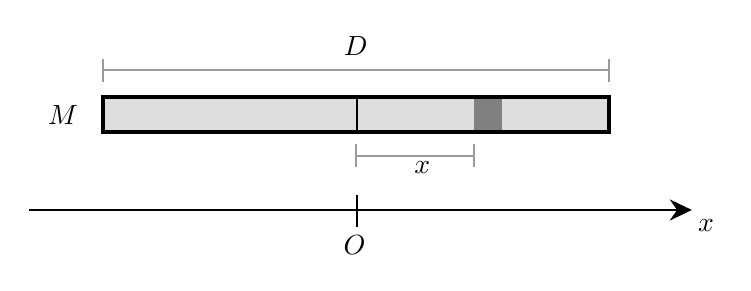
\begin{tikzpicture}[x=0.75pt,y=0.75pt,yscale=-1,xscale=1]
	%uncomment if require: \path (0,300); %set diagram left start at 0, and has height of 300

	%Straight Lines [id:da6939231860886572] 
	\draw    (161,211) -- (477.5,211) ;
	\draw [shift={(480.5,211)}, rotate = 180] [fill={rgb, 255:red, 0; green, 0; blue, 0 }  ][line width=0.08]  [draw opacity=0] (10.72,-5.15) -- (0,0) -- (10.72,5.15) -- (7.12,0) -- cycle    ;
	%Straight Lines [id:da49746209378373907] 
	\draw    (319,204) -- (319,219) ;
	%Shape: Rectangle [id:dp023827527134408832] 
	\draw  [draw opacity=0][fill={rgb, 255:red, 222; green, 222; blue, 222 }  ,fill opacity=1 ][line width=1.5]  (196.67,156.67) -- (440.67,156.67) -- (440.67,173.33) -- (196.67,173.33) -- cycle ;
	%Straight Lines [id:da04830795019727763] 
	\draw [color={rgb, 255:red, 155; green, 155; blue, 155 }  ,draw opacity=1 ]   (196.67,143.67) -- (440.67,143.67) ;
	\draw [shift={(440.67,143.67)}, rotate = 180] [color={rgb, 255:red, 155; green, 155; blue, 155 }  ,draw opacity=1 ][line width=0.75]    (0,5.59) -- (0,-5.59)   ;
	\draw [shift={(196.67,143.67)}, rotate = 180] [color={rgb, 255:red, 155; green, 155; blue, 155 }  ,draw opacity=1 ][line width=0.75]    (0,5.59) -- (0,-5.59)   ;
	%Straight Lines [id:da9433065630599604] 
	\draw    (319,157) -- (319,173.29) ;
	%Shape: Rectangle [id:dp9291189988064272] 
	\draw  [draw opacity=0][fill={rgb, 255:red, 128; green, 128; blue, 128 }  ,fill opacity=1 ] (375.4,156.67) -- (389.13,156.67) -- (389.13,173.33) -- (375.4,173.33) -- cycle ;
	%Straight Lines [id:da7586638771789609] 
	\draw [color={rgb, 255:red, 155; green, 155; blue, 155 }  ,draw opacity=1 ]   (318.67,184.8) -- (375.67,184.8) ;
	\draw [shift={(375.67,184.8)}, rotate = 180] [color={rgb, 255:red, 155; green, 155; blue, 155 }  ,draw opacity=1 ][line width=0.75]    (0,5.59) -- (0,-5.59)   ;
	\draw [shift={(318.67,184.8)}, rotate = 180] [color={rgb, 255:red, 155; green, 155; blue, 155 }  ,draw opacity=1 ][line width=0.75]    (0,5.59) -- (0,-5.59)   ;
	%Shape: Rectangle [id:dp7061108287025681] 
	\draw  [line width=1.5]  (196.67,156.67) -- (440.67,156.67) -- (440.67,173.33) -- (196.67,173.33) -- cycle ;

	% Text Node
	\draw (318,227.67) node    {$O$};
	% Text Node
	\draw (487.33,218.33) node    {$x$};
	% Text Node
	\draw (318.5,132.17) node    {$D$};
	% Text Node
	\draw (350.63,190.67) node  [font=\normalsize]  {$x$};
	% Text Node
	\draw (177.5,165.17) node    {$M$};

	\end{tikzpicture}
\end{figure}
\FloatBarrier
Per definire la distanza assiale di una generica massa $i$-esima si definisce un asse parallelo alla lunghezza dell'asta. L'origine la si pone in corrispondente all'asse. La distanza assiale è proprio la variabile $x$. Si ha $dm=\lambda dx$.

\[
	I_z = \int_{-D/2}^{D/2} dm\,x^2 = \int_{-D/2}^{D/2} \lambda x^2 dx
\]

Diamo per scontato che l'asta sia omogenea, quindi con densità lineare costante $\lambda=M/D$.

\[
	I_z = \frac{M}{D} \left[ \frac{x^3 }{3} \right]_{-D/2}^{D/2} = \frac{M}{3D}\frac{D^3 }{8}2 = \frac{1}{12}MD^2
\]

Se la stessa asta la si fa ruotare intorno a un asse $z$ passante per l'estremo dell'asta, $I_z$ aumenta perché si ha più massa lontana dall'asse di rotazione.

\[
	I_z = \int_0^D dm\,x^2 = \frac{M}{D}\left[ \frac{x^2 }{3} \right]_0^D = \frac{M}{D}\frac{D^3 }{3}= \frac{1}{3} MD^2
\]

\paragraph{La macchina di Atwood} Si cerca in questo esempio di capire come delle forze provocano l'accelerazione angolare del corpo rigido.

\begin{figure}[htpb]
	\centering

	\tikzset{every picture/.style={line width=0.75pt}} %set default line width to 0.75pt        

	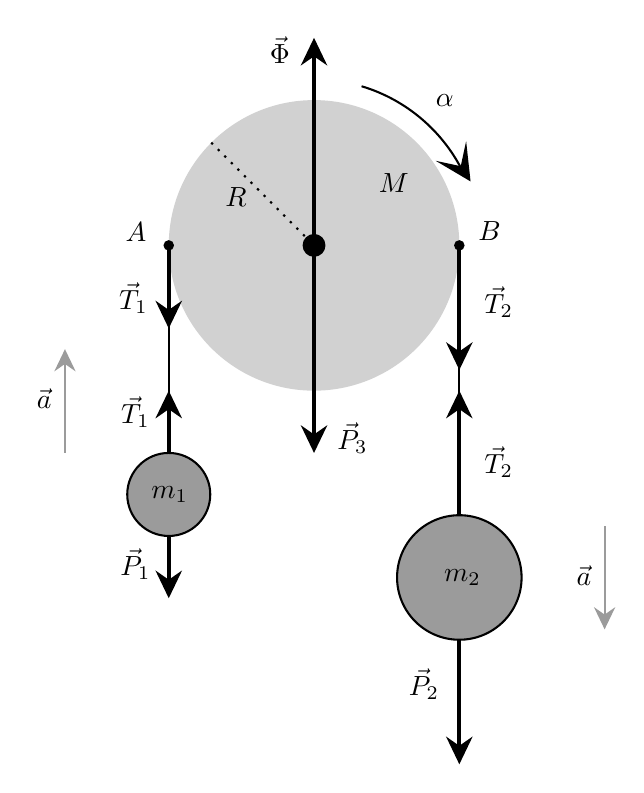
\begin{tikzpicture}[x=0.75pt,y=0.75pt,yscale=-1,xscale=1]
	%uncomment if require: \path (0,476); %set diagram left start at 0, and has height of 476

	%Shape: Circle [id:dp287190602871209] 
	\draw  [draw opacity=0][fill={rgb, 255:red, 209; green, 209; blue, 209 }  ,fill opacity=1 ] (231,187) .. controls (231,148.34) and (262.34,117) .. (301,117) .. controls (339.66,117) and (371,148.34) .. (371,187) .. controls (371,225.66) and (339.66,257) .. (301,257) .. controls (262.34,257) and (231,225.66) .. (231,187) -- cycle ;
	%Shape: Circle [id:dp577091868880393] 
	\draw  [fill={rgb, 255:red, 155; green, 155; blue, 155 }  ,fill opacity=1 ] (341,347) .. controls (341,330.43) and (354.43,317) .. (371,317) .. controls (387.57,317) and (401,330.43) .. (401,347) .. controls (401,363.57) and (387.57,377) .. (371,377) .. controls (354.43,377) and (341,363.57) .. (341,347) -- cycle ;
	%Shape: Circle [id:dp7005266442079385] 
	\draw  [fill={rgb, 255:red, 155; green, 155; blue, 155 }  ,fill opacity=1 ] (211,307) .. controls (211,295.95) and (219.95,287) .. (231,287) .. controls (242.05,287) and (251,295.95) .. (251,307) .. controls (251,318.05) and (242.05,327) .. (231,327) .. controls (219.95,327) and (211,318.05) .. (211,307) -- cycle ;
	%Straight Lines [id:da31695538097494946] 
	\draw    (231,187) -- (231,287) ;
	%Straight Lines [id:da7585268171258928] 
	\draw    (371,187) -- (371,317) ;
	%Straight Lines [id:da32083901818240124] 
	\draw [line width=1.5]    (301,187) -- (301,91) ;
	\draw [shift={(301,87)}, rotate = 450] [fill={rgb, 255:red, 0; green, 0; blue, 0 }  ][line width=0.08]  [draw opacity=0] (13.4,-6.43) -- (0,0) -- (13.4,6.44) -- (8.9,0) -- cycle    ;
	%Straight Lines [id:da5376464248095933] 
	\draw [line width=1.5]    (301,187) -- (301,283) ;
	\draw [shift={(301,287)}, rotate = 270] [fill={rgb, 255:red, 0; green, 0; blue, 0 }  ][line width=0.08]  [draw opacity=0] (13.4,-6.43) -- (0,0) -- (13.4,6.44) -- (8.9,0) -- cycle    ;
	%Shape: Circle [id:dp10748121142795108] 
	\draw  [fill={rgb, 255:red, 0; green, 0; blue, 0 }  ,fill opacity=1 ] (296,187) .. controls (296,184.24) and (298.24,182) .. (301,182) .. controls (303.76,182) and (306,184.24) .. (306,187) .. controls (306,189.76) and (303.76,192) .. (301,192) .. controls (298.24,192) and (296,189.76) .. (296,187) -- cycle ;
	%Straight Lines [id:da3684136627430463] 
	\draw [line width=1.5]    (371,187) -- (371,243) ;
	\draw [shift={(371,247)}, rotate = 270] [fill={rgb, 255:red, 0; green, 0; blue, 0 }  ][line width=0.08]  [draw opacity=0] (13.4,-6.43) -- (0,0) -- (13.4,6.44) -- (8.9,0) -- cycle    ;
	%Straight Lines [id:da18692534139299388] 
	\draw [line width=1.5]    (371,317) -- (371,261) ;
	\draw [shift={(371,257)}, rotate = 450] [fill={rgb, 255:red, 0; green, 0; blue, 0 }  ][line width=0.08]  [draw opacity=0] (13.4,-6.43) -- (0,0) -- (13.4,6.44) -- (8.9,0) -- cycle    ;
	%Straight Lines [id:da10085015388066632] 
	\draw [line width=1.5]    (231,187) -- (231,223) ;
	\draw [shift={(231,227)}, rotate = 270] [fill={rgb, 255:red, 0; green, 0; blue, 0 }  ][line width=0.08]  [draw opacity=0] (13.4,-6.43) -- (0,0) -- (13.4,6.44) -- (8.9,0) -- cycle    ;
	%Straight Lines [id:da8881358901703795] 
	\draw [line width=1.5]    (231,287) -- (231,261) ;
	\draw [shift={(231,257)}, rotate = 450] [fill={rgb, 255:red, 0; green, 0; blue, 0 }  ][line width=0.08]  [draw opacity=0] (13.4,-6.43) -- (0,0) -- (13.4,6.44) -- (8.9,0) -- cycle    ;
	%Straight Lines [id:da4824151405818853] 
	\draw [line width=1.5]    (231,353) -- (231,327) ;
	\draw [shift={(231,357)}, rotate = 270] [fill={rgb, 255:red, 0; green, 0; blue, 0 }  ][line width=0.08]  [draw opacity=0] (13.4,-6.43) -- (0,0) -- (13.4,6.44) -- (8.9,0) -- cycle    ;
	%Straight Lines [id:da17712756501560833] 
	\draw [line width=1.5]    (371,433) -- (371,377) ;
	\draw [shift={(371,437)}, rotate = 270] [fill={rgb, 255:red, 0; green, 0; blue, 0 }  ][line width=0.08]  [draw opacity=0] (13.4,-6.43) -- (0,0) -- (13.4,6.44) -- (8.9,0) -- cycle    ;
	%Straight Lines [id:da049600524167557225] 
	\draw [color={rgb, 255:red, 155; green, 155; blue, 155 }  ,draw opacity=1 ][line width=0.75]    (181,287) -- (181,240) ;
	\draw [shift={(181,237)}, rotate = 450] [fill={rgb, 255:red, 155; green, 155; blue, 155 }  ,fill opacity=1 ][line width=0.08]  [draw opacity=0] (10.72,-5.15) -- (0,0) -- (10.72,5.15) -- (7.12,0) -- cycle    ;
	%Straight Lines [id:da43365541795855966] 
	\draw [color={rgb, 255:red, 155; green, 155; blue, 155 }  ,draw opacity=1 ][line width=0.75]    (441,369) -- (441,322) ;
	\draw [shift={(441,372)}, rotate = 270] [fill={rgb, 255:red, 155; green, 155; blue, 155 }  ,fill opacity=1 ][line width=0.08]  [draw opacity=0] (10.72,-5.15) -- (0,0) -- (10.72,5.15) -- (7.12,0) -- cycle    ;
	%Shape: Arc [id:dp041555453597121206] 
	\draw  [draw opacity=0] (323.9,110.33) .. controls (345.63,116.81) and (363.48,132.27) .. (373.15,152.4) -- (301,187) -- cycle ; \draw   (323.9,110.33) .. controls (345.63,116.81) and (363.48,132.27) .. (373.15,152.4) ;
	\draw  [fill={rgb, 255:red, 0; green, 0; blue, 0 }  ,fill opacity=1 ] (374.12,139.89) -- (375.81,155.25) -- (362.51,147.38) -- (372.06,149.45) -- cycle ;
	%Shape: Circle [id:dp6438603490091646] 
	\draw  [fill={rgb, 255:red, 0; green, 0; blue, 0 }  ,fill opacity=1 ] (229,187) .. controls (229,185.9) and (229.9,185) .. (231,185) .. controls (232.1,185) and (233,185.9) .. (233,187) .. controls (233,188.1) and (232.1,189) .. (231,189) .. controls (229.9,189) and (229,188.1) .. (229,187) -- cycle ;
	%Shape: Circle [id:dp25257009832339206] 
	\draw  [fill={rgb, 255:red, 0; green, 0; blue, 0 }  ,fill opacity=1 ] (369,187) .. controls (369,185.9) and (369.9,185) .. (371,185) .. controls (372.1,185) and (373,185.9) .. (373,187) .. controls (373,188.1) and (372.1,189) .. (371,189) .. controls (369.9,189) and (369,188.1) .. (369,187) -- cycle ;
	%Straight Lines [id:da996236735362686] 
	\draw [line width=0.75]  [dash pattern={on 0.84pt off 2.51pt}]  (251.5,137.5) -- (301,187) ;

	% Text Node
	\draw (339.4,157) node    {$M$};
	% Text Node
	\draw (284.5,93) node    {$\vec{\Phi }$};
	% Text Node
	\draw (319.5,279.8) node    {$\vec{P}_{3}$};
	% Text Node
	\draw (390,214.5) node    {$\vec{T}_{2}$};
	% Text Node
	\draw (390,291.5) node    {$\vec{T}_{2}$};
	% Text Node
	\draw (214,212.5) node    {$\vec{T}_{1}$};
	% Text Node
	\draw (215,267.5) node    {$\vec{T}_{1}$};
	% Text Node
	\draw (231.5,307) node    {$m_{1}$};
	% Text Node
	\draw (372.5,347) node    {$m_{2}$};
	% Text Node
	\draw (215,340.5) node    {$\vec{P}_{1}$};
	% Text Node
	\draw (354,398.5) node    {$\vec{P}_{2}$};
	% Text Node
	\draw (171,261) node    {$\vec{a}$};
	% Text Node
	\draw (431,346) node    {$\vec{a}$};
	% Text Node
	\draw (364,117) node    {$\alpha $};
	% Text Node
	\draw (215.2,180.4) node    {$A$};
	% Text Node
	\draw (385.6,180) node    {$B$};
	% Text Node
	\draw (263.4,163.8) node    {$R$};

	\end{tikzpicture}
\end{figure}
\FloatBarrier
La macchina di Atwood è semplicemente una carrucola: essa è costituita da due oggetti di massa $m_1$ e $m_2$ connessi da un filo inestensibile posto sopra una carrucola. Essa è pesante, ha una sua inerzia e per essere messa in rotazione richiede una certa forza. La carrucola è un disco di massa $M$ e raggio $R$ che viene vincolata rispetto al suo centro e può ruotare intorno ad esso. Questo vuole dire che allora essa potrà ruotare intorno all'asse $z$ ortogonale al piano del foglio passante per il centro della carrucola. Essa da ferma si mette ad accelerare in verso orario. $m_1$ sale e $m_2$ scende. La fune è di massa trascurabile e quindi l'accelerazione per tutti i punti, anche quella dei due corpi, è la stessa. Il corpo di massa $m_1$ vorrebbe cadere verso il basso a causa della forza peso ma è sostenuto dalla tensione della fune che lo porta verso l'alto.

\[
	T_1 - m_1 g = m_1 a
\]

Analogamente $m_2$ è mossa verso il basso dalla forza peso e sostenuta dalla tensione della fune. Si avrà:

\[
	m_2 g - T_2 = m_2 a
\]
$m_1$ genera la tensione $\vec{T}_1$. Si sa che essa si propaga inalterata fino al punto A della carrucola. Essa vorrebbe essere spinta verso il basso dalla tensione $\vec{T}_1$. D'altra parte anche sul corpo $m_2$ agisce $\vec{T}_2$ che si propaga inalterata fino a $B$. Per il principio di azione e reazione si vede che la carrucola è soggetta anche ad una tensione $\vec{T}_2$. Si consideri nel disegno solo le forze applicate alla carrucola. C'è una reazione vincolare generata dall'asse, dal sostegno che fa in modo che la carrucola rimanga ferma, non cada. Queste sono le uniche forze applicate ad essa. Si noti che sono state impostate le tensioni diverse. Se le tensioni fossero uguali la carrucola non ruoterebbe. Se il corpo in rotazione è dotato di massa, la sua inerzia fa variare la tensione della fune.

Si impone il fatto che le forze si devono bilanciare in verticale:

\[
	R_{tot} = 0 \implies \Phi - T_1 - T_2 - Mg = 0
\]

Si calcolano i momenti di tutte le forze in direzione assiale.

\[
	M_z = T_2 R - T_1 R = I_z\alpha
\]

Il legame che manca fra le relazioni scritte per poter risolvere il problema è che l'accelerazione angolare non è indipendente dall'accelerazione lineare con cui si muovono i corpi. Aggiungendo l'informazione che $a=\alpha R$, si risolve il sistema.

\begin{gather*}
	T_2\frac{R}{R} - T_1 \frac{R}{R} =  \frac{I_z \alpha  }{R} \\
	m_2 g - m_1 g = (m_1+m_2)\alpha R + \frac{I_z\alpha  }{R}
\end{gather*}

\[
	\boxed{\alpha = \frac{g(m_2-m_1)}{m_1+m_2+ \frac{I_z }{R^2}}\frac{1}{R}}
\]

Il sistema ha una accelerazione angolare $\alpha$ pari a quella trovata.

Si immagini di avere un corpo esteso che questa volta si guarda dall'alto in modo tale che l'asse attorno a cui ruota è ortogonale al piano del foglio.

\begin{figure}[htpb]
	\centering

	\tikzset{every picture/.style={line width=0.75pt}} %set default line width to 0.75pt        

	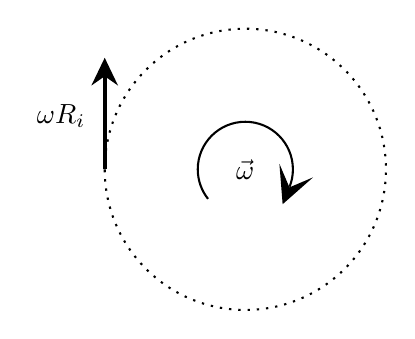
\begin{tikzpicture}[x=0.75pt,y=0.75pt,yscale=-1,xscale=1]
	%uncomment if require: \path (0,300); %set diagram left start at 0, and has height of 300

	%Shape: Circle [id:dp07436427005931256] 
	\draw  [dash pattern={on 0.84pt off 2.51pt}] (193,144.75) .. controls (193,107.33) and (223.33,77) .. (260.75,77) .. controls (298.17,77) and (328.5,107.33) .. (328.5,144.75) .. controls (328.5,182.17) and (298.17,212.5) .. (260.75,212.5) .. controls (223.33,212.5) and (193,182.17) .. (193,144.75) -- cycle ;
	%Straight Lines [id:da9965818127873434] 
	\draw [line width=1.5]    (193,144.75) -- (193,95) ;
	\draw [shift={(193,91)}, rotate = 450] [fill={rgb, 255:red, 0; green, 0; blue, 0 }  ][line width=0.08]  [draw opacity=0] (13.4,-6.43) -- (0,0) -- (13.4,6.44) -- (8.9,0) -- cycle    ;
	\draw  [fill={rgb, 255:red, 0; green, 0; blue, 0 }  ,fill opacity=1 ] (290.73,150.29) -- (279.14,160.52) -- (277.91,145.12) -- (281.73,154.11) -- cycle ;
	%Shape: Arc [id:dp8802504072717734] 
	\draw  [draw opacity=0] (242.78,158.98) .. controls (239.68,155.07) and (237.83,150.12) .. (237.83,144.75) .. controls (237.83,132.09) and (248.09,121.83) .. (260.75,121.83) .. controls (273.41,121.83) and (283.67,132.09) .. (283.67,144.75) .. controls (283.67,147.72) and (283.1,150.55) .. (282.08,153.15) -- (260.75,144.75) -- cycle ; \draw   (242.78,158.98) .. controls (239.68,155.07) and (237.83,150.12) .. (237.83,144.75) .. controls (237.83,132.09) and (248.09,121.83) .. (260.75,121.83) .. controls (273.41,121.83) and (283.67,132.09) .. (283.67,144.75) .. controls (283.67,147.72) and (283.1,150.55) .. (282.08,153.15) ;

	% Text Node
	\draw (172,119.17) node    {$\omega R_{i}$};
	% Text Node
	\draw (260.75,144.75) node    {$\vec{\omega }$};

	\end{tikzpicture}
\end{figure}
\FloatBarrier
In questo tipo di moto tutti i punti si muovono con la stessa velocità angolare $\omega$ che sarà un vettore parallelo all'asse $z$. Si sottolinea che se si prende un generico punto $i$ del corpo, esso ha velocità vettoriale tangente alla circonferenza e con modulo pari a $\omega R_i$. Questa informazione è importante perché se il corpo è collegato ad altri corpi, bisogna capire come la sua velocità si collega alle altre. Se si vuole che un corpo che sta ruotando con una certa $\omega$ vari la sua velocità angolare, è necessario che agiscano su di esso delle forze che danno luogo a dei momenti diretti parallelamente all'asse di rotazione. Il legame tra l'azione dinamica e l'effetto cinematico è la seconda equazione cardinale della dinamica per un corpo in rotazione intorno a un asse $z$.

\[
	M_z = I_z \alpha
\]

Dove il momento di inerzia rappresenta l'inerzia che il corpo oppone alla variazione della sua velocità angolare. Se si vuole che $\omega$ sia una funzione del tempo, è necessario che esistano dei momenti assiali. Se questi momenti non esistono, o si compensano a vicenda, si ha che il momento angolare totale, e in particolare quello assiale, sarà costante. Questo vuole dire che, presi due istanti di tempo successivi, ci sono due possibilità:

\begin{itemize}
	\item il corpo ha momento di inerzia che non varia durante il movimento e dunque, se i momenti assiali sono nulli o si bilanciano, esso si muove di moto rotatorio uniforme.
	\item se durante il moto per qualche motivo varia il momento di inerzia del corpo, si mantiene costante il prodotto tra il momento di inerzia e la velocità angolare. Se per qualche motivo il corpo aumenta il momento di inerzia, avviene che diminuisce la sua velocità angolare. Se per un punto materiale non è così naturale pensare che cambi la sua massa, per un corpo può accadere che il momento di inerzia vari perché la massa viene spostata da una parte all'altra del corpo.
	\[
		M_z^{(o)} = 0 \implies \vec{L}^{(o)} = \text{costante} = I_z\omega
	\]
\end{itemize}

Ora ci si chiede se la prima equazione cardinale della dinamica serva per studiare il moto di rotazione di un corpo intorno a un asse fisso. Si noti che se l'asse $z$ non passa per il centro di massa, quest'ultimo non è fermo ma deve ruotare anche lui su una circonferenza con raggio $R$ e centro sull'asse $z$. Mi aspetto che la prima equazione cardinale della dinamica mi dia un valore non nullo, che ci siano forze che fanno muovere il centro di massa. Se invece si fa coincidere l'asse $z$ con il centro di massa, ci si aspetta che il centro di massa sia fermo e che tale equazione dica che la risultante delle forze è nulla. Si può studiare il moto del corpo usando le due equazioni cardinali della dinamica o sostituendo una delle due con il teorema dell'energia cinetica.

\section{Energia cinetica di un corpo in rotazione}

L'energia cinetica è data da:

\[
	\sum_i \frac{1}{2} m_i v_i^2 = \sum_i \frac{1}{2} m_i\omega^2 R_i^2  = \frac{1}{2} \omega^2 \left( \sum_i m_i^2 R_i^2 \right)
\]

Il termine tra parentesi è proprio il momento di inerzia. Quindi si ottiene un'espressione che definisce l'energia cinetica di un corpo che ruota intorno all'asse $z$. Bisogna fare attenzione al fatto che il momento di inerzia è quello del corpo \emph{rispetto all'asse di rotazione}, \emph{non} rispetto al centro di massa.

\[
	E_K=\frac{1}{2} I_z\omega^2
\]

Se si hanno delle forze che generano dei momenti, bisogna capire come si scrive il lavoro delle forze quando queste invece che far traslare un punto del sistema lo fanno ruotare, quindi il lavoro dei momenti delle forze.

\begin{figure}[htpb]
	\centering

	\tikzset{every picture/.style={line width=0.75pt}} %set default line width to 0.75pt        

	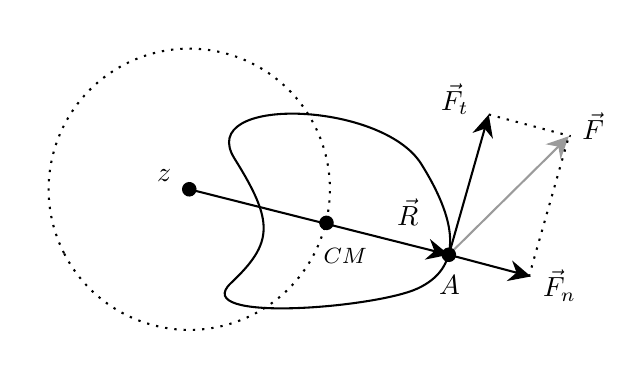
\begin{tikzpicture}[x=0.75pt,y=0.75pt,yscale=-1,xscale=1]
	%uncomment if require: \path (0,300); %set diagram left start at 0, and has height of 300

	%Straight Lines [id:da7037828027851607] 
	\draw [color={rgb, 255:red, 155; green, 155; blue, 155 }  ,draw opacity=1 ]   (356.55,188.52) -- (412.24,133.53) ;
	\draw [shift={(414.38,131.42)}, rotate = 495.36] [fill={rgb, 255:red, 155; green, 155; blue, 155 }  ,fill opacity=1 ][line width=0.08]  [draw opacity=0] (10.72,-5.15) -- (0,0) -- (10.72,5.15) -- (7.12,0) -- cycle    ;
	%Shape: Regular Polygon [id:dp7869409182664271] 
	\draw   (341.52,204.77) .. controls (321.24,214.19) and (230.99,221.59) .. (251.56,202.17) .. controls (272.13,182.76) and (272.41,172.76) .. (253.29,142.2) .. controls (234.16,111.64) and (324.12,114.23) .. (343.25,144.79) .. controls (362.38,175.35) and (361.8,195.35) .. (341.52,204.77) -- cycle ;
	%Shape: Circle [id:dp009598075955776997] 
	\draw  [dash pattern={on 0.84pt off 2.51pt}] (171.11,187.72) .. controls (154.13,154.38) and (167.39,113.58) .. (200.74,96.6) .. controls (234.08,79.62) and (274.87,92.88) .. (291.85,126.22) .. controls (308.84,159.57) and (295.57,200.36) .. (262.23,217.34) .. controls (228.89,234.32) and (188.09,221.06) .. (171.11,187.72) -- cycle ;
	%Shape: Circle [id:dp5400712793990026] 
	\draw  [fill={rgb, 255:red, 0; green, 0; blue, 0 }  ,fill opacity=1 ] (228.81,158.33) .. controls (228.06,156.86) and (228.65,155.05) .. (230.12,154.3) .. controls (231.6,153.55) and (233.41,154.13) .. (234.16,155.61) .. controls (234.91,157.09) and (234.32,158.89) .. (232.85,159.65) .. controls (231.37,160.4) and (229.56,159.81) .. (228.81,158.33) -- cycle ;
	%Straight Lines [id:da11086399310222395] 
	\draw    (231.48,156.97) -- (353.64,187.79) ;
	\draw [shift={(356.55,188.52)}, rotate = 194.16] [fill={rgb, 255:red, 0; green, 0; blue, 0 }  ][line width=0.08]  [draw opacity=0] (10.72,-5.15) -- (0,0) -- (10.72,5.15) -- (7.12,0) -- cycle    ;
	%Shape: Circle [id:dp663064867078651] 
	\draw  [fill={rgb, 255:red, 0; green, 0; blue, 0 }  ,fill opacity=1 ] (294.92,174.53) .. controls (294.17,173.05) and (294.76,171.25) .. (296.24,170.5) .. controls (297.71,169.74) and (299.52,170.33) .. (300.27,171.81) .. controls (301.02,173.28) and (300.44,175.09) .. (298.96,175.84) .. controls (297.48,176.59) and (295.68,176.01) .. (294.92,174.53) -- cycle ;
	%Shape: Circle [id:dp02478333726937576] 
	\draw  [fill={rgb, 255:red, 0; green, 0; blue, 0 }  ,fill opacity=1 ] (353.88,189.89) .. controls (353.12,188.41) and (353.71,186.6) .. (355.19,185.85) .. controls (356.66,185.1) and (358.47,185.69) .. (359.22,187.16) .. controls (359.97,188.64) and (359.39,190.45) .. (357.91,191.2) .. controls (356.43,191.95) and (354.63,191.36) .. (353.88,189.89) -- cycle ;
	%Straight Lines [id:da6728968637253481] 
	\draw    (356.55,188.52) -- (393.15,198.21) ;
	\draw [shift={(396.05,198.98)}, rotate = 194.83] [fill={rgb, 255:red, 0; green, 0; blue, 0 }  ][line width=0.08]  [draw opacity=0] (10.72,-5.15) -- (0,0) -- (10.72,5.15) -- (7.12,0) -- cycle    ;
	%Straight Lines [id:da7741385010148079] 
	\draw    (356.55,188.52) -- (374.95,123.83) ;
	\draw [shift={(375.77,120.95)}, rotate = 465.88] [fill={rgb, 255:red, 0; green, 0; blue, 0 }  ][line width=0.08]  [draw opacity=0] (10.72,-5.15) -- (0,0) -- (10.72,5.15) -- (7.12,0) -- cycle    ;
	%Straight Lines [id:da8723315686748525] 
	\draw  [dash pattern={on 0.84pt off 2.51pt}]  (375.77,120.95) -- (415.27,131.4) ;
	%Straight Lines [id:da6197450263799631] 
	\draw  [dash pattern={on 0.84pt off 2.51pt}]  (395.15,199) -- (414.38,131.42) ;

	% Text Node
	\draw (219.4,150.58) node    {$z$};
	% Text Node
	\draw (306.62,189.09) node  [font=\footnotesize]  {$CM$};
	% Text Node
	\draw (336.78,168.15) node    {$\vec{R}$};
	% Text Node
	\draw (356.88,203.11) node    {$A$};
	% Text Node
	\draw (359.45,113.74) node    {$\vec{F}_{t}$};
	% Text Node
	\draw (426.15,126.55) node    {$\vec{F}$};
	% Text Node
	\draw (409.89,203.42) node    {$\vec{F}_{n}$};

	\end{tikzpicture}
\end{figure}
\FloatBarrier
Si immagini che per far ruotare il corpo agisca su $A$ la forza $\vec{F}$. Tale punto si muove sull'archetto di circonferenza con centro sull'asse $z$, di lunghezza $ds$. La componente della forza che compie lavoro è solo quella tangente alla circonferenza. Si può trasformare lo spostamento lineare del punto in uno spostamento angolare $d\vartheta$, dove $ds = R\,d\vartheta$. Ma $\vec{F}_t R$ non è altro che l'intensità del momento generato dalla forza $F$ rispetto al polo $z$. Lo si chiama $\vec{M}_z$, ed è il momento assiale che permette al corpo di ruotare. Con queste informazioni, si scrive il lavoro compiuto da $\vec{F}$:

\[
	\mathcal{L} = \int \vec{F}_t \cdot d\vec{s} = \int F_t Rd\vartheta = \int M_z d\vartheta
\]

Note le intensità dei momenti assiali, il lavoro dei momenti si calcola proprio come: $\mathcal{L} = \int M_z d\vartheta$. Con queste ultime due informazioni trovate, si può applicare il teorema dell'energia cinetica, che fa vedere l'effetto dal punto di vista energetico del lavoro compiuto dalle forze. Si andrà a sostituire alla relazione $M=I\alpha$ perché collega l'effetto dei momenti delle forze all'accelerazione del corpo o alla variazione di energia cinetica.

\textbf{I principali momenti di inerzia}

\begin{itemize}

	\item \textbf{Anello} che ruota attorno al suo centro di massa $\boxed{I_z = MR^2}$

	\item \textbf{Disco} che ruota attorno al suo centro $\boxed{I_z=\frac{1}{2} MR^2}$

	\item \textbf{Cilindro} che ruota attorno al suo asse. Il suo momento di inerzia è esattamente lo stesso di quello del disco. Questo perché la massa non ha cambiato la sua distribuzione rispetto all'asse $z$ ma è solo stata distribuita lungo una direzione. $\boxed{I_z = \frac{1}{2} MR^2}$

	\item \textbf{Guscio cilindrico sottile} che ruota attorno al suo asse. Analogo discorso varrebbe per l'anello. Se si considera un guscio cilindrico sottile, il suo momento sarà sempre $\boxed{I_z = MR^2}$

	\item \textbf{Sfera} di raggio $R$. Una sfera, fatta ruotare per un qualunque asse passante per il suo centro, avrà momento di inerzia inferiore a quello del cilindro perché ho maggiore massa distribuita più lontano dall'asse $z$ nel caso del cilindro. $\boxed{I_z = \frac{2}{5}MR^2}$

	\item \textbf{Asta} di lunghezza $L$ che ruota intorno ad un asse $z$ passante per il suo centro $\boxed{I_z = \frac{1}{12}ML^2}$

	\item \textbf{Lastra}  di lati $A$ e $B$ che ruota attorno al suo centro: $\boxed{I_z = \frac{1}{12}M(A^2+B^2)}$
\end{itemize}

\section{Teorema di Huygens-Steiner}

Se si fa ruotare il disco rispetto a un altro asse, non passante per forza per il centro di massa,  viene in aiuto il \textbf{teorema degli assi paralleli}, o teorema di Huygens-Steiner. Si supponga di avere un corpo di forma qualunque di cui è noto il momento di inerzia rispetto a un asse $z'$ passante per il centro di massa. Il teorema degli assi paralleli permette di calcolare il momento di inerzia del corpo rispetto a un qualunque altro asse $z \parallel z'$. Il teorema afferma che nota la distanza assiale tra i due assi, $D$, e la massa $M$ del corpo, il momento di inerzia di esso rispetto all'asse $z$ sarà calcolabile partendo dal momento di inerzia rispetto a $z'$, in aggiunta a una quantità sempre positiva data dalla massa del corpo per il quadrato della distanza fra i due corpi:

\[
	\boxed{I_z = I_{z'} + MD^2, \quad I_z > I_{z'}}
\]

Qualunque sia l'asse $z$, il momento di inerzia è sempre maggiore rispetto a quello rispetto all'asse passante per il centro di massa, $z'$.

\begin{figure}[htpb]
	\centering

	\tikzset{every picture/.style={line width=0.75pt}} %set default line width to 0.75pt        

	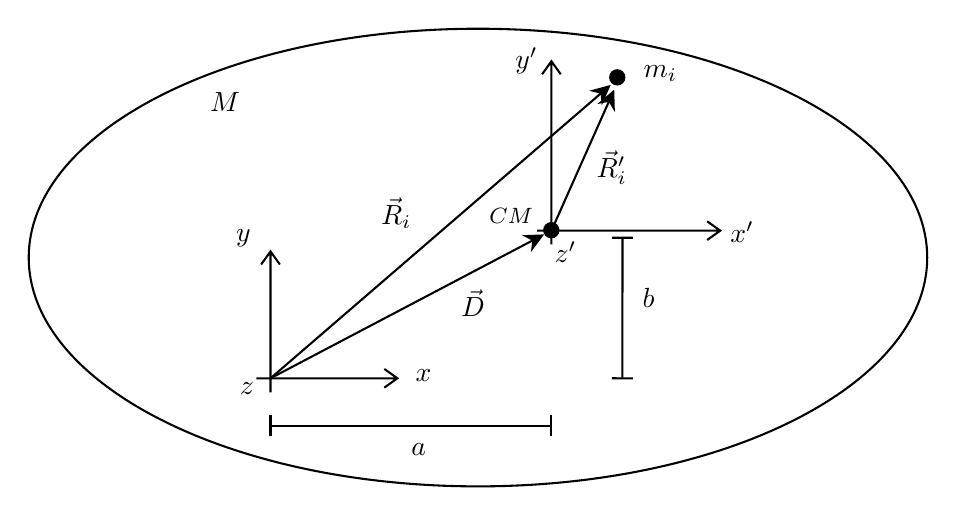
\begin{tikzpicture}[x=0.75pt,y=0.75pt,yscale=-0.9,xscale=0.9]
	%uncomment if require: \path (0,300); %set diagram left start at 0, and has height of 300

	%Shape: Axis 2D [id:dp8273336417410213] 
	\draw  (148.9,220.64) -- (224.37,220.64)(156.44,152.71) -- (156.44,228.18) (217.37,215.64) -- (224.37,220.64) -- (217.37,225.64) (151.44,159.71) -- (156.44,152.71) -- (161.44,159.71)  ;
	%Shape: Axis 2D [id:dp46760875552896186] 
	\draw  (299.21,141.61) -- (397.2,141.61)(306.82,50.91) -- (306.82,148.9) (390.2,136.61) -- (397.2,141.61) -- (390.2,146.61) (301.82,57.91) -- (306.82,50.91) -- (311.82,57.91)  ;
	%Shape: Circle [id:dp33560493835936445] 
	\draw  [fill={rgb, 255:red, 0; green, 0; blue, 0 }  ,fill opacity=1 ] (302.95,141.36) .. controls (302.95,139.25) and (304.66,137.55) .. (306.76,137.55) .. controls (308.86,137.55) and (310.57,139.25) .. (310.57,141.36) .. controls (310.57,143.46) and (308.86,145.16) .. (306.76,145.16) .. controls (304.66,145.16) and (302.95,143.46) .. (302.95,141.36) -- cycle ;
	%Shape: Ellipse [id:dp07615770474265449] 
	\draw  [fill={rgb, 255:red, 0; green, 0; blue, 0 }  ,fill opacity=1 ] (338.26,59.54) .. controls (338.26,57.44) and (339.96,55.73) .. (342.07,55.73) .. controls (344.17,55.73) and (345.87,57.44) .. (345.87,59.54) .. controls (345.87,61.64) and (344.17,63.34) .. (342.07,63.34) .. controls (339.96,63.34) and (338.26,61.64) .. (338.26,59.54) -- cycle ;
	%Straight Lines [id:da39168454837719757] 
	\draw    (156.44,220.64) -- (300.27,145) ;
	\draw [shift={(302.92,143.61)}, rotate = 512.26] [fill={rgb, 255:red, 0; green, 0; blue, 0 }  ][line width=0.08]  [draw opacity=0] (10.72,-5.15) -- (0,0) -- (10.72,5.15) -- (7.12,0) -- cycle    ;
	%Straight Lines [id:da9139176154510034] 
	\draw    (156.44,220.64) -- (336.26,65.56) ;
	\draw [shift={(338.54,63.6)}, rotate = 499.22] [fill={rgb, 255:red, 0; green, 0; blue, 0 }  ][line width=0.08]  [draw opacity=0] (10.72,-5.15) -- (0,0) -- (10.72,5.15) -- (7.12,0) -- cycle    ;
	%Shape: Ellipse [id:dp30294253521760495] 
	\draw   (27,156) .. controls (27,88.35) and (134.68,33.5) .. (267.5,33.5) .. controls (400.32,33.5) and (508,88.35) .. (508,156) .. controls (508,223.65) and (400.32,278.5) .. (267.5,278.5) .. controls (134.68,278.5) and (27,223.65) .. (27,156) -- cycle ;
	%Straight Lines [id:da30583034209389814] 
	\draw    (306.82,141.61) -- (339.22,68.87) ;
	\draw [shift={(340.44,66.13)}, rotate = 474.01] [fill={rgb, 255:red, 0; green, 0; blue, 0 }  ][line width=0.08]  [draw opacity=0] (10.72,-5.15) -- (0,0) -- (10.72,5.15) -- (7.12,0) -- cycle    ;
	%Straight Lines [id:da6744668858852887] 
	\draw    (156.44,246.01) -- (306.76,246.01) ;
	\draw [shift={(306.76,246.01)}, rotate = 180] [color={rgb, 255:red, 0; green, 0; blue, 0 }  ][line width=0.75]    (0,5.59) -- (0,-5.59)   ;
	\draw [shift={(156.44,246.01)}, rotate = 180] [color={rgb, 255:red, 0; green, 0; blue, 0 }  ][line width=0.75]    (0,5.59) -- (0,-5.59)   ;
	%Straight Lines [id:da8072781954268866] 
	\draw    (344.81,220.64) -- (344.88,145.41) ;
	\draw [shift={(344.88,145.41)}, rotate = 450.05] [color={rgb, 255:red, 0; green, 0; blue, 0 }  ][line width=0.75]    (0,5.59) -- (0,-5.59)   ;
	\draw [shift={(344.81,220.64)}, rotate = 450.05] [color={rgb, 255:red, 0; green, 0; blue, 0 }  ][line width=0.75]    (0,5.59) -- (0,-5.59)   ;

	% Text Node
	\draw (238.32,219.3) node    {$x$};
	% Text Node
	\draw (141.92,145.73) node    {$y$};
	% Text Node
	\draw (143.82,226.28) node    {$z$};
	% Text Node
	\draw (408.94,142.56) node    {$x'$};
	% Text Node
	\draw (293.5,50.59) node    {$y'$};
	% Text Node
	\draw (314.37,153.28) node    {$z'$};
	% Text Node
	\draw (264.87,180.58) node    {$\vec{D}$};
	% Text Node
	\draw (365.17,57.57) node    {$m_{i}$};
	% Text Node
	\draw (285.26,133.68) node  [font=\footnotesize]  {$CM$};
	% Text Node
	\draw (223.74,132.41) node    {$\vec{R}_{i}$};
	% Text Node
	\draw (339.17,107.68) node    {$\vec{R} '_{i}$};
	% Text Node
	\draw (235.79,258.63) node    {$a$};
	% Text Node
	\draw (358.83,177.44) node    {$b$};
	% Text Node
	\draw (132.17,72.57) node    {$M$};

	\end{tikzpicture}
\end{figure}
\FloatBarrier

\paragraph{Dimostrazione} Si definisce un sistema di riferimento centrato sul centro di massa con assi $x', y'$ e $z'$ e un sistema di riferimento centrato sul punto rispetto al quale si vuole calcolare il momento di inerzia, $x, y, z$.
Nota $D$, siano:

\begin{itemize}
	\item $a=$ ascissa della distanza fra i due sistemi di riferimento;
	\item $b=$ distanza in termini di ordinata fra i due sistemi di riferimento.
\end{itemize}

Per prima cosa si applica la definizione di momento di inerzia, utilizzando la notazione discreta. Si immagini di suddividere il corpo in tante masse infinitesime. Il momento di inerzia sarà la somma della massa $i$-esima per il quadrato della distanza assiale fra la massa $i$-esima e l'asse. $R_i$ si può riscrivere come:

\[
	R_i^2 = x_i^2 + y_i^2
\]

Dove $x_i$ e $y_i$ sono l'ascissa e l'ordinata della massa $i$-esima rispetto al sistema di riferimento centrato nell'asse $z$. Siano $x_i'$ e $y_i'$ le coordinate della massa $i$-esima rispetto all'altro sistema di riferimento.

\[
	\sum_i m_i x_i^2  = \sum_i m_i (x_i'+a)^2 = \sum_i m_i x_i'^2 + \sum_i m_i a^2 + \sum_i 2 a m_i x_i'
\]

Per quanto riguarda l'ultimo termine, si noti che $2a$ lo posso portare fuori dalla sommatoria. La sommatoria darebbe luogo a:

\[
	\sum_i m_i x_i'
\]

Si tratta della massa del sistema per l'ascissa del centro di massa nel sistema di riferimento del centro di massa, pertanto non può che essere $0$. Si usa lo stesso concetto utilizzato per il teorema di K\"onig.

\begin{equation*}
	\begin{aligned}
		\sum_i m_i x_i^2 &= \sum_i m_i x_i'^2 + \sum_i m_i a^2 \\
		\sum_i m_i y_i^2 &= \sum_i m_i y_i'^2 + \sum_i m_i b^2 \\
		\\
		I_z &= \sum_i m_i R_i^2 \\
		&= \sum_i m_i x_i^2 + \sum_i m_i y_i^2 \\
		&=\sum_i m_i x_i'^2 + \sum_i m_i a^2 + \sum_i m_i y_i'^2 + \sum_i m_i b^2 \\
		&= \sum_i m_i R_i'^2 +\sum_i m_i D^2 \\
		&= I_z' + MD^2 \\
	\end{aligned}
\end{equation*}

Si ottiene così ciò che si voleva dimostrare.

\subsection{Confronto fra il teorema di Huygens Steiner e di K\"onig}

Dal momento che si ha utilizzato un ragionamento analogo per il teorema di K\"onig, si deduce che esso ha fondamentalmente lo stesso significato e fornisce le stesse informazioni. L'energia cinetica del corpo rigido in rotazione sarà data da:

\[
	E_K = \frac{1}{2} \omega^2 I_z
\]

Si definisce un asse $z'$ parallelo a $z$ e passante per il centro di massa e si va a sostituire le informazioni fornite dal teorema di Huygens-Steiner.

\[
	E_K = \frac{1}{2} \omega^2 (I_z' + MD^2) = \frac{1}{2} \omega^2 I_z' + \frac{1}{2} \omega^2 MD^2
\]

Il primo termine è l'energia cinetica di un corpo che sta ruotando intorno all'asse $z'$ rispetto al centro di massa. Per quanto riguarda il secondo termine, si ha $\omega D$, che dimensionalmente è una velocità lineare di un punto che ruota su una circonferenza di raggio $D$. In particolare esso sarà il centro di massa. Quindi il secondo termine si può scrivere meglio come:

\[
	\frac{1}{2} M(D\omega)^2 = \frac{1}{2} Mv_{cm}^2
\]

Dunque:

\[
	E_K = \underbrace{\frac{1}{2} \omega^2 I_z'}_{E_K\text{ rotazione attorno al }cm  } + \underbrace{\frac{1}{2} Mv_{cm}^2}_{E_K\text{ traslazione } cm }
\]

Questi due contributi sono quelli che sono nati quando è stato enunciato e dimostrato il teorema di K\"onig.

\paragraph{Esempio di applicazione del teorema dell'energia cinetica} Si immagini di avere un disco che è fissato intorno al suo centro in modo tale che possa ruotare intorno ad esso.

\begin{figure}[htpb]
	\centering

	\tikzset{every picture/.style={line width=0.75pt}} %set default line width to 0.75pt        

	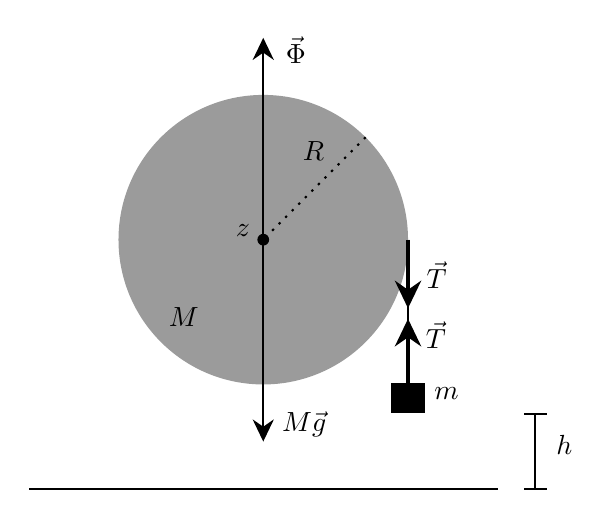
\begin{tikzpicture}[x=0.75pt,y=0.75pt,yscale=-1,xscale=1]
	%uncomment if require: \path (0,300); %set diagram left start at 0, and has height of 300

	%Shape: Circle [id:dp37449881724298395] 
	\draw  [draw opacity=0][fill={rgb, 255:red, 155; green, 155; blue, 155 }  ,fill opacity=1 ] (237,136.75) .. controls (237,98.23) and (268.23,67) .. (306.75,67) .. controls (345.27,67) and (376.5,98.23) .. (376.5,136.75) .. controls (376.5,175.27) and (345.27,206.5) .. (306.75,206.5) .. controls (268.23,206.5) and (237,175.27) .. (237,136.75) -- cycle ;
	%Straight Lines [id:da3587624434409662] 
	\draw    (306.75,136.75) -- (306.75,231) ;
	\draw [shift={(306.75,234)}, rotate = 270] [fill={rgb, 255:red, 0; green, 0; blue, 0 }  ][line width=0.08]  [draw opacity=0] (10.72,-5.15) -- (0,0) -- (10.72,5.15) -- (7.12,0) -- cycle    ;
	%Straight Lines [id:da3594545535993927] 
	\draw    (306.75,42.5) -- (306.75,136.75) ;
	\draw [shift={(306.75,39.5)}, rotate = 90] [fill={rgb, 255:red, 0; green, 0; blue, 0 }  ][line width=0.08]  [draw opacity=0] (10.72,-5.15) -- (0,0) -- (10.72,5.15) -- (7.12,0) -- cycle    ;
	%Shape: Circle [id:dp6298373522875735] 
	\draw  [draw opacity=0][fill={rgb, 255:red, 0; green, 0; blue, 0 }  ,fill opacity=1 ] (303.92,136.75) .. controls (303.92,135.19) and (305.19,133.92) .. (306.75,133.92) .. controls (308.31,133.92) and (309.58,135.19) .. (309.58,136.75) .. controls (309.58,138.31) and (308.31,139.58) .. (306.75,139.58) .. controls (305.19,139.58) and (303.92,138.31) .. (303.92,136.75) -- cycle ;
	%Straight Lines [id:da6804063707082968] 
	\draw    (376.5,136.75) -- (376.5,213) ;
	%Shape: Rectangle [id:dp7253125564821739] 
	\draw  [fill={rgb, 255:red, 0; green, 0; blue, 0 }  ,fill opacity=1 ] (368.83,206.33) -- (384.17,206.33) -- (384.17,219.67) -- (368.83,219.67) -- cycle ;
	%Straight Lines [id:da5070125564426535] 
	\draw [line width=1.5]    (376.5,136.75) -- (376.5,165.8) ;
	\draw [shift={(376.5,169.8)}, rotate = 270] [fill={rgb, 255:red, 0; green, 0; blue, 0 }  ][line width=0.08]  [draw opacity=0] (13.4,-6.43) -- (0,0) -- (13.4,6.44) -- (8.9,0) -- cycle    ;
	%Straight Lines [id:da3741592651594814] 
	\draw [line width=1.5]    (376.5,178.88) -- (376.5,207.93) ;
	\draw [shift={(376.5,174.88)}, rotate = 90] [fill={rgb, 255:red, 0; green, 0; blue, 0 }  ][line width=0.08]  [draw opacity=0] (13.4,-6.43) -- (0,0) -- (13.4,6.44) -- (8.9,0) -- cycle    ;
	%Straight Lines [id:da8878387068216638] 
	\draw  [dash pattern={on 0.84pt off 2.51pt}]  (356.07,87.43) -- (306.75,136.75) ;
	%Straight Lines [id:da25441565817973344] 
	\draw    (419.75,256.75) -- (193.75,256.75) ;
	%Straight Lines [id:da588260612497469] 
	\draw    (437.75,220.67) -- (437.75,256.75) ;
	\draw [shift={(437.75,256.75)}, rotate = 270] [color={rgb, 255:red, 0; green, 0; blue, 0 }  ][line width=0.75]    (0,5.59) -- (0,-5.59)   ;
	\draw [shift={(437.75,220.67)}, rotate = 270] [color={rgb, 255:red, 0; green, 0; blue, 0 }  ][line width=0.75]    (0,5.59) -- (0,-5.59)   ;

	% Text Node
	\draw (297,132.5) node    {$z$};
	% Text Node
	\draw (322.5,45.5) node    {$\vec{\Phi }$};
	% Text Node
	\draw (326.5,225.5) node    {$M\vec{g}$};
	% Text Node
	\draw (395.1,211.1) node    {$m$};
	% Text Node
	\draw (390.3,153.7) node    {$\vec{T}$};
	% Text Node
	\draw (389.9,182.9) node    {$\vec{T}$};
	% Text Node
	\draw (331,93.83) node    {$R$};
	% Text Node
	\draw (268.5,174.17) node    {$M$};
	% Text Node
	\draw (451.83,235.5) node    {$h$};

	\end{tikzpicture}
\end{figure}
\FloatBarrier
Intorno al cilindro è avvolto un filo al cui estremo è applicata la massa $m$, a una quota $h$ dal suolo: inizialmente essa è sostenuta. Il sostegno viene rimosso e si vuole sapere con che velocità esso arriva al suolo.
Sul rocchetto agiranno sicuramente la forza peso, il vincolo che non lo fa cadere a terra e la tensione del filo. Mentre queste due forze non compiono lavoro, la tensione lo farà. In particolare darà un momento $TR$. Esso deve servire per far variare l'energia cinetica del rocchetto. Il tutto lo si lega alla variazione di quota di $m$, che arriverà al suolo con un'energia potenziale nulla. $mgh$ non si trasforma interamente in energia cinetica perché così la massa si comporterebbe come se fosse libera. Ma non è così, la massa per cadere verso il basso deve muovere questo disco che ha una sua inerzia. C'è una forza che agisce sulla massa che è la tensione del filo.

\paragraph{Esempio del pendolo composto} È un esempio interessante del moto di rotazione di un corpo rigido attorno a un asse.

\begin{figure}[htpb]
	\centering

	\tikzset{every picture/.style={line width=0.75pt}} %set default line width to 0.75pt        

	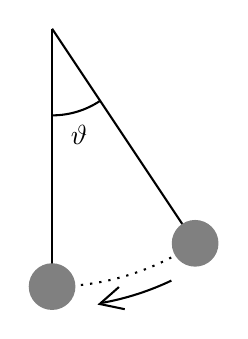
\begin{tikzpicture}[x=0.75pt,y=0.75pt,yscale=-1,xscale=1]
	%uncomment if require: \path (0,300); %set diagram left start at 0, and has height of 300

	%Shape: Arc [id:dp25219748707798706] 
	\draw  [draw opacity=0][dash pattern={on 0.84pt off 2.51pt}] (365.43,199.39) .. controls (345.71,212.57) and (322,220.25) .. (296.5,220.25) -- (296.5,96) -- cycle ; \draw  [dash pattern={on 0.84pt off 2.51pt}] (365.43,199.39) .. controls (345.71,212.57) and (322,220.25) .. (296.5,220.25) ;
	%Straight Lines [id:da6360552694564299] 
	\draw    (296.5,96) -- (296.5,221) ;
	%Straight Lines [id:da6954033748497943] 
	\draw    (296.5,96) -- (365.43,199.39) ;
	%Shape: Arc [id:dp5035601333805273] 
	\draw  [draw opacity=0] (319.66,130.74) .. controls (313.03,135.17) and (305.07,137.75) .. (296.5,137.75) -- (296.5,96) -- cycle ; \draw   (319.66,130.74) .. controls (313.03,135.17) and (305.07,137.75) .. (296.5,137.75) ;
	%Shape: Circle [id:dp45991567118054166] 
	\draw  [draw opacity=0][fill={rgb, 255:red, 128; green, 128; blue, 128 }  ,fill opacity=1 ] (285.25,220.25) .. controls (285.25,214.04) and (290.29,209) .. (296.5,209) .. controls (302.71,209) and (307.75,214.04) .. (307.75,220.25) .. controls (307.75,226.46) and (302.71,231.5) .. (296.5,231.5) .. controls (290.29,231.5) and (285.25,226.46) .. (285.25,220.25) -- cycle ;
	%Shape: Circle [id:dp9187145095922711] 
	\draw  [draw opacity=0][fill={rgb, 255:red, 128; green, 128; blue, 128 }  ,fill opacity=1 ] (354.18,199.39) .. controls (354.18,193.18) and (359.22,188.14) .. (365.43,188.14) .. controls (371.64,188.14) and (376.68,193.18) .. (376.68,199.39) .. controls (376.68,205.61) and (371.64,210.64) .. (365.43,210.64) .. controls (359.22,210.64) and (354.18,205.61) .. (354.18,199.39) -- cycle ;
	%Shape: Arc [id:dp06123254472319295] 
	\draw  [draw opacity=0] (353.97,217.36) .. controls (343.53,222.32) and (332.34,225.96) .. (320.62,228.09) -- (296.5,96) -- cycle ; \draw   (353.97,217.36) .. controls (343.53,222.32) and (332.34,225.96) .. (320.62,228.09) ;
	\draw   (331.53,231.13) -- (319.45,228.63) -- (328.7,220.47) ;

	% Text Node
	\draw (309.5,147) node    {$\vartheta $};

	\end{tikzpicture}
\end{figure}
\FloatBarrier
Nel pendolo composto la massa non è puntiforme ma è un corpo esteso che viene fatto oscillare, vincolato ad un certo punto. Si ha che la posizione di equilibrio del corpo è sulla verticale. Il movimento sarà dato sempre dalla forza peso, che tende a riportare il corpo nella posizione di equilibrio. Bisogna però risolvere il problema
utilizzando l'equazione dei momenti e tenendo conto dell'inerzia del sistema.

\section{Il moto di rototraslazione}

Il moto di rototraslazione è quello caratteristico di un corpo che ruota e intanto trasla. Il modo più comodo per studiarlo è quello di vederlo come combinazione della rotazione del corpo attorno al centro di massa più la traslazione di quest'ultimo. Si può anche considerarlo come la rotazione attorno a un qualsiasi punto del corpo più la traslazione di questo. Si utilizza la prima equazione cardinale della dinamica per studiare il moto di traslazione del centro di massa e la seconda equazione cardinale della dinamica per studiare la rotazione.

\paragraph{Moto di scivolamento senza slittamento} Si tratta di un particolare caso di rototraslazione. È il moto di un oggetto che può rotolare su un piano in modo tale che mentre rotola, il punto di contatto con il piano d'appoggio non slitta mai. Si consideri un disco di raggio $R$ che rotola senza strisciare su un piano d'appoggio orizzontale.

\begin{figure}[htpb]
	\centering

	% Pattern Info
	 
	\tikzset{
	pattern size/.store in=\mcSize, 
	pattern size = 5pt,
	pattern thickness/.store in=\mcThickness, 
	pattern thickness = 0.3pt,
	pattern radius/.store in=\mcRadius, 
	pattern radius = 1pt}
	\makeatletter
	\pgfutil@ifundefined{pgf@pattern@name@_mwikyhy1d}{
	\pgfdeclarepatternformonly[\mcThickness,\mcSize]{_mwikyhy1d}
	{\pgfqpoint{0pt}{0pt}}
	{\pgfpoint{\mcSize+\mcThickness}{\mcSize+\mcThickness}}
	{\pgfpoint{\mcSize}{\mcSize}}
	{
	\pgfsetcolor{\tikz@pattern@color}
	\pgfsetlinewidth{\mcThickness}
	\pgfpathmoveto{\pgfqpoint{0pt}{0pt}}
	\pgfpathlineto{\pgfpoint{\mcSize+\mcThickness}{\mcSize+\mcThickness}}
	\pgfusepath{stroke}
	}}
	\makeatother
	\tikzset{every picture/.style={line width=0.75pt}} %set default line width to 0.75pt        

	\begin{tikzpicture}[x=0.75pt,y=0.75pt,yscale=-1,xscale=1]
	%uncomment if require: \path (0,300); %set diagram left start at 0, and has height of 300

	%Shape: Rectangle [id:dp05787029687722711] 
	\draw  [draw opacity=0][pattern=_mwikyhy1d,pattern size=6pt,pattern thickness=0.75pt,pattern radius=0pt, pattern color={rgb, 255:red, 155; green, 155; blue, 155}] (180,210) -- (462.75,210) -- (462.75,225.5) -- (180,225.5) -- cycle ;
	%Straight Lines [id:da9575884425325174] 
	\draw    (180,210) -- (470.5,210) ;
	\draw [shift={(473.5,210)}, rotate = 180] [fill={rgb, 255:red, 0; green, 0; blue, 0 }  ][line width=0.08]  [draw opacity=0] (10.72,-5.15) -- (0,0) -- (10.72,5.15) -- (7.12,0) -- cycle    ;
	%Shape: Circle [id:dp6173822162539673] 
	\draw   (210,165) .. controls (210,140.15) and (230.15,120) .. (255,120) .. controls (279.85,120) and (300,140.15) .. (300,165) .. controls (300,189.85) and (279.85,210) .. (255,210) .. controls (230.15,210) and (210,189.85) .. (210,165) -- cycle ;
	%Shape: Circle [id:dp31313922768748026] 
	\draw  [dash pattern={on 0.84pt off 2.51pt}] (340,165) .. controls (340,140.15) and (360.15,120) .. (385,120) .. controls (409.85,120) and (430,140.15) .. (430,165) .. controls (430,189.85) and (409.85,210) .. (385,210) .. controls (360.15,210) and (340,189.85) .. (340,165) -- cycle ;
	%Straight Lines [id:da010485267518391517] 
	\draw    (255,165) -- (281.17,128.33) ;
	%Shape: Arc [id:dp5132535481287805] 
	\draw  [draw opacity=0] (264.99,111.31) .. controls (276.67,113.47) and (287.05,119.35) .. (294.85,127.68) -- (255,165) -- cycle ; \draw   (264.99,111.31) .. controls (276.67,113.47) and (287.05,119.35) .. (294.85,127.68) ;
	\draw   (291.33,117.34) -- (295.67,128.25) -- (284.34,125.17) ;
	%Shape: Circle [id:dp15806679768486953] 
	\draw  [fill={rgb, 255:red, 0; green, 0; blue, 0 }  ,fill opacity=1 ] (252.25,210) .. controls (252.25,208.48) and (253.48,207.25) .. (255,207.25) .. controls (256.52,207.25) and (257.75,208.48) .. (257.75,210) .. controls (257.75,211.52) and (256.52,212.75) .. (255,212.75) .. controls (253.48,212.75) and (252.25,211.52) .. (252.25,210) -- cycle ;
	%Shape: Circle [id:dp45395702869368915] 
	\draw  [fill={rgb, 255:red, 0; green, 0; blue, 0 }  ,fill opacity=1 ] (382.25,210) .. controls (382.25,208.48) and (383.48,207.25) .. (385,207.25) .. controls (386.52,207.25) and (387.75,208.48) .. (387.75,210) .. controls (387.75,211.52) and (386.52,212.75) .. (385,212.75) .. controls (383.48,212.75) and (382.25,211.52) .. (382.25,210) -- cycle ;

	% Text Node
	\draw (263.2,136) node    {$R$};
	% Text Node
	\draw (283.45,101.75) node    {$\vec{\omega }$};
	% Text Node
	\draw (246.5,192.5) node    {$C$};
	% Text Node
	\draw (377.5,194) node    {$C$};

	\end{tikzpicture}
\end{figure}
\FloatBarrier
I vari punti sulla circonferenza via via nel movimento andranno a contatto con il suolo. Quello che succede è che il punto del corpo che era a contatto con il suolo, $C$, che ovviamente cambierà istante per istante, perché non strisci deve avere istantaneamente velocità nulla. Se il corpo rotola senza strisciare, le varie parti del corpo avranno una velocità, ma $C$ istantaneamente si ferma. Si noti che il corpo non sta ruotando attorno all'asse passante per il centro di massa ma attorno all'asse $z$ passante per il punto di contatto, che via via cambia durante il moto. I vari punti del corpo, a parte il centro di massa, che si sposta parallelamente al piano di appoggio, seguono traiettorie più complicate di quelle viste finora.

\begin{figure}[htpb]
	\centering

	% Pattern Info
	 
	\tikzset{
	pattern size/.store in=\mcSize, 
	pattern size = 5pt,
	pattern thickness/.store in=\mcThickness, 
	pattern thickness = 0.3pt,
	pattern radius/.store in=\mcRadius, 
	pattern radius = 1pt}
	\makeatletter
	\pgfutil@ifundefined{pgf@pattern@name@_ghnoqj5wk}{
	\pgfdeclarepatternformonly[\mcThickness,\mcSize]{_ghnoqj5wk}
	{\pgfqpoint{0pt}{0pt}}
	{\pgfpoint{\mcSize+\mcThickness}{\mcSize+\mcThickness}}
	{\pgfpoint{\mcSize}{\mcSize}}
	{
	\pgfsetcolor{\tikz@pattern@color}
	\pgfsetlinewidth{\mcThickness}
	\pgfpathmoveto{\pgfqpoint{0pt}{0pt}}
	\pgfpathlineto{\pgfpoint{\mcSize+\mcThickness}{\mcSize+\mcThickness}}
	\pgfusepath{stroke}
	}}
	\makeatother
	\tikzset{every picture/.style={line width=0.75pt}} %set default line width to 0.75pt        

	\begin{tikzpicture}[x=0.75pt,y=0.75pt,yscale=-1,xscale=1]
	%uncomment if require: \path (0,300); %set diagram left start at 0, and has height of 300

	%Shape: Rectangle [id:dp14507808096786023] 
	\draw  [draw opacity=0][pattern=_ghnoqj5wk,pattern size=6pt,pattern thickness=0.75pt,pattern radius=0pt, pattern color={rgb, 255:red, 155; green, 155; blue, 155}] (130,210) -- (485.75,210) -- (485.75,226) -- (130,226) -- cycle ;
	%Straight Lines [id:da9852040206440102] 
	\draw    (130,210) -- (497,210) ;
	\draw [shift={(500,210)}, rotate = 180] [fill={rgb, 255:red, 0; green, 0; blue, 0 }  ][line width=0.08]  [draw opacity=0] (10.72,-5.15) -- (0,0) -- (10.72,5.15) -- (7.12,0) -- cycle    ;
	%Shape: Circle [id:dp13866972663201427] 
	\draw   (160,175) .. controls (160,155.67) and (175.67,140) .. (195,140) .. controls (214.33,140) and (230,155.67) .. (230,175) .. controls (230,194.33) and (214.33,210) .. (195,210) .. controls (175.67,210) and (160,194.33) .. (160,175) -- cycle ;
	%Shape: Circle [id:dp6026450717164555] 
	\draw   (270,175) .. controls (270,155.67) and (285.67,140) .. (305,140) .. controls (324.33,140) and (340,155.67) .. (340,175) .. controls (340,194.33) and (324.33,210) .. (305,210) .. controls (285.67,210) and (270,194.33) .. (270,175) -- cycle ;
	%Shape: Circle [id:dp0024488836516574075] 
	\draw   (380,175) .. controls (380,155.67) and (395.67,140) .. (415,140) .. controls (434.33,140) and (450,155.67) .. (450,175) .. controls (450,194.33) and (434.33,210) .. (415,210) .. controls (395.67,210) and (380,194.33) .. (380,175) -- cycle ;
	%Curve Lines [id:da1351197624789504] 
	\draw [line width=1.5]    (195,140) .. controls (260.75,140.5) and (290.25,180.5) .. (305,210) ;
	%Curve Lines [id:da2535479529176272] 
	\draw [line width=1.5]    (415,140) .. controls (351.25,140) and (320.25,180.5) .. (305,210) ;
	%Shape: Circle [id:dp12598589167302587] 
	\draw  [fill={rgb, 255:red, 0; green, 0; blue, 0 }  ,fill opacity=1 ] (302.25,209) .. controls (302.25,207.48) and (303.48,206.25) .. (305,206.25) .. controls (306.52,206.25) and (307.75,207.48) .. (307.75,209) .. controls (307.75,210.52) and (306.52,211.75) .. (305,211.75) .. controls (303.48,211.75) and (302.25,210.52) .. (302.25,209) -- cycle ;

	% Text Node
	\draw (304,188) node    {$C$};

	\end{tikzpicture}
\end{figure}
\FloatBarrier
In un moto di rototraslazione, la velocità di un generico punto del corpo si può sempre vedere come la velocità del centro di massa, più la velocità dovuta alla rotazione del punto intorno al centro di massa:

\[
	\vec{v} (P) = \vec{v}_{cm} + \vec{\omega}\times \vec{r}_{cm}(P)
\]

Si sfrutta questa relazione per capire il legame tra la velocità del punto di contatto $C$ e la velocità del centro di massa.

\[
	\vec{v} (C) = \vec{v}_{cm} + \vec{\omega}\times \vec{r}_{cm}(C)
\]
$\vec{\omega}\times \vec{r}_{cm}(C)$ è un vettore parallelo al piano d'appoggio diretto a sinistra (il senso è orario).

\[
	\vec{\omega} \times \vec{r}(C) = -\omega R \vec{u}_x
\]

La velocità di $C$ in un moto di rotolamento senza strisciamento vale zero. Imporre che la velocità del punto di contatto sia uguale a zero istantaneamente, vuole dire imporre che il centro di massa abbia una velocità strettamente legata alla velocità angolare di rotazione perché vale $\omega R$.

\[
	\boxed{v_{cm} = \omega R}
\]

Se si pensava di avere due incognite in un moto di rototraslazione, in realtà questa relazione fa avere una sola incognita,  basta trovare $\omega$ e si ricava anche la velocità con cui si muove il centro di massa. Nel moto di puro rotolamento infatti, la velocità di rotazione e quella di traslazione non sono indipendenti.
Si capisce perché il moto può essere visto come il moto di rotazione attorno al punto di contatto. I punti che devono compiere spazio maggiore sono quelli sul perimetro, il centro di massa si muove meno, il punto di contatto invece non si muove. Il modo più conveniente è quello di vederlo come un moto di rotazione attorno al punto di contatto, istantaneamente fermo.

\paragraph{Esempio} Per fare in modo che le ruote di un'automobile quando ruotano non slittino, è necessario che ci sia un piano d'appoggio con sufficiente attrito da bloccare il punto di contatto, che deve essere istantaneamente fermo. Si tratterà di forza di attrito statico, e sarà diretta in direzione tangente al moto, facendo ruotare il corpo. Ad esempio, se si applica una forza $\vec{F}_o$ al centro del disco di intensità costante e tangente al piano, l'oggetto non riesce a slittare ma grazie all'attrito può rotolare. Potrebbe anche succedere che, invece che cercare di far muovere l'oggetto tirandolo, gli si applica un motore di rotazione, una coppia motrice. Si tratta di una coppia di forze uguali e opposte che non ha l'effetto di traslare ma di mettere in rotazione. In questo caso l'oggetto tenderà a ruotare indietro e allora la forza di attrito statico risulterà diretto in avanti. Le forze che agiscono sul corpo sono quelle
in figura.

\begin{figure}[htpb]
	\centering

	\tikzset{every picture/.style={line width=0.75pt}} %set default line width to 0.75pt        

	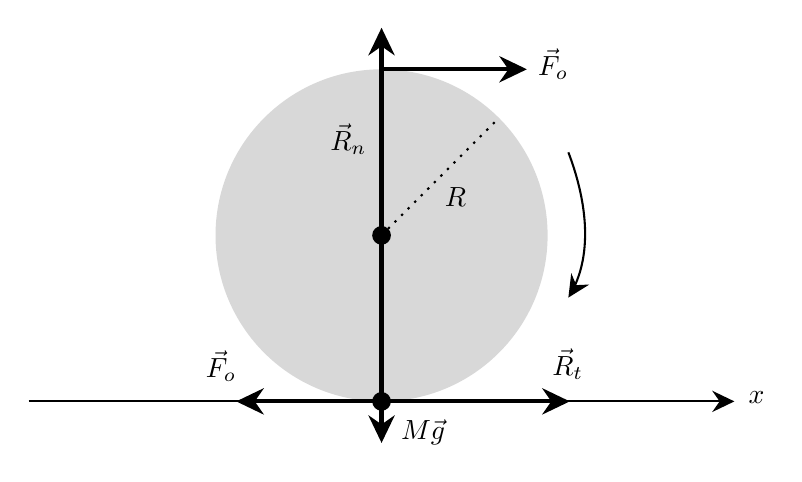
\begin{tikzpicture}[x=0.75pt,y=0.75pt,yscale=-1,xscale=1]
	%uncomment if require: \path (0,300); %set diagram left start at 0, and has height of 300

	%Straight Lines [id:da6140945885120805] 
	\draw    (100,240) -- (437,240) ;
	\draw [shift={(440,240)}, rotate = 180] [fill={rgb, 255:red, 0; green, 0; blue, 0 }  ][line width=0.08]  [draw opacity=0] (10.72,-5.15) -- (0,0) -- (10.72,5.15) -- (7.12,0) -- cycle    ;
	%Shape: Circle [id:dp2872045225708375] 
	\draw  [draw opacity=0][fill={rgb, 255:red, 216; green, 216; blue, 216 }  ,fill opacity=1 ] (190,160) .. controls (190,115.82) and (225.82,80) .. (270,80) .. controls (314.18,80) and (350,115.82) .. (350,160) .. controls (350,204.18) and (314.18,240) .. (270,240) .. controls (225.82,240) and (190,204.18) .. (190,160) -- cycle ;
	%Straight Lines [id:da507849495249439] 
	\draw [line width=1.5]    (270,160) -- (270,64) ;
	\draw [shift={(270,60)}, rotate = 450] [fill={rgb, 255:red, 0; green, 0; blue, 0 }  ][line width=0.08]  [draw opacity=0] (13.4,-6.43) -- (0,0) -- (13.4,6.44) -- (8.9,0) -- cycle    ;
	%Shape: Circle [id:dp4881888290360934] 
	\draw  [fill={rgb, 255:red, 0; green, 0; blue, 0 }  ,fill opacity=1 ] (266,160) .. controls (266,157.79) and (267.79,156) .. (270,156) .. controls (272.21,156) and (274,157.79) .. (274,160) .. controls (274,162.21) and (272.21,164) .. (270,164) .. controls (267.79,164) and (266,162.21) .. (266,160) -- cycle ;
	%Straight Lines [id:da21324584280345382] 
	\draw [line width=1.5]    (270,256) -- (270,160) ;
	\draw [shift={(270,260)}, rotate = 270] [fill={rgb, 255:red, 0; green, 0; blue, 0 }  ][line width=0.08]  [draw opacity=0] (13.4,-6.43) -- (0,0) -- (13.4,6.44) -- (8.9,0) -- cycle    ;
	%Straight Lines [id:da9034182639606498] 
	\draw [line width=1.5]    (204,240) -- (270,240) ;
	\draw [shift={(200,240)}, rotate = 0] [fill={rgb, 255:red, 0; green, 0; blue, 0 }  ][line width=0.08]  [draw opacity=0] (13.4,-6.43) -- (0,0) -- (13.4,6.44) -- (8.9,0) -- cycle    ;
	%Straight Lines [id:da7554370242670971] 
	\draw [line width=1.5]    (270,80) -- (336,80) ;
	\draw [shift={(340,80)}, rotate = 180] [fill={rgb, 255:red, 0; green, 0; blue, 0 }  ][line width=0.08]  [draw opacity=0] (13.4,-6.43) -- (0,0) -- (13.4,6.44) -- (8.9,0) -- cycle    ;
	%Curve Lines [id:da21076727837307252] 
	\draw    (360,120) .. controls (368.32,141.76) and (372.34,167.82) .. (361.44,187.57) ;
	\draw [shift={(360,190)}, rotate = 302.35] [fill={rgb, 255:red, 0; green, 0; blue, 0 }  ][line width=0.08]  [draw opacity=0] (10.72,-5.15) -- (0,0) -- (10.72,5.15) -- (7.12,0) -- cycle    ;
	%Straight Lines [id:da050615307129076026] 
	\draw [line width=1.5]    (270,240) -- (356.67,240) ;
	\draw [shift={(360.67,240)}, rotate = 180] [fill={rgb, 255:red, 0; green, 0; blue, 0 }  ][line width=0.08]  [draw opacity=0] (13.4,-6.43) -- (0,0) -- (13.4,6.44) -- (8.9,0) -- cycle    ;
	%Shape: Circle [id:dp11678220559527897] 
	\draw  [fill={rgb, 255:red, 0; green, 0; blue, 0 }  ,fill opacity=1 ] (266,240) .. controls (266,237.79) and (267.79,236) .. (270,236) .. controls (272.21,236) and (274,237.79) .. (274,240) .. controls (274,242.21) and (272.21,244) .. (270,244) .. controls (267.79,244) and (266,242.21) .. (266,240) -- cycle ;
	%Straight Lines [id:da6964104143677115] 
	\draw [line width=0.75]  [dash pattern={on 0.84pt off 2.51pt}]  (270,160) -- (326.57,103.43) ;

	% Text Node
	\draw (450.67,238.33) node    {$x$};
	% Text Node
	\draw (290,255) node    {$M\vec{g}$};
	% Text Node
	\draw (254,113.67) node    {$\vec{R}_{n}$};
	% Text Node
	\draw (359.67,222) node    {$\vec{R}_{t}$};
	% Text Node
	\draw (352.67,77.67) node    {$\vec{F}_{o}$};
	% Text Node
	\draw (192.67,223) node    {$\vec{F}_{o}$};
	% Text Node
	\draw (305.67,141.33) node    {$R$};

	\end{tikzpicture}
\end{figure}
\FloatBarrier
Applicare una coppia di forze di questo tipo è equivalente a applicare un momento $M_z$ esterno di intensità $2 F_o R$. Applicando la prima e la seconda legge cardinale della dinamica:

\[
	\begin{array}{rl}
		\text{I equazione} & \left\{\begin{array}{l}
									 	x:\quad R_t=Ma_{cm}  \\
										y:\quad Mg = R_n
									\end{array} \right. \\ \\
		\text{II equazione} & M_z = I_z\alpha
	\end{array}
\]

Si cosideri un asse $z$ passante per $C$, lo si sceglie con verso entrante nel piano del foglio. Rispetto al polo $C$, l'unica forza che genera momento è $\vec{F}_o$ (sopra). Il suo momento sarà:

\[
	M_z = F_o\cdot 2R = I_z\alpha \qquad \alpha = \frac{F_o 2 R}{I_z }
\]

Il momento di inerzia non è riferito all'asse passante per il centro di massa, ma per il teorema di Huygens-Steiner, sarà:

\[
	I_z = \frac{1}{2} MR^2 + MR^2 = \frac{3}{2} MR^2 \qquad \alpha = \frac{F_o 4 R}{3MR^2} = \frac{4}{3}\frac{F_o }{MR}
\]

Il piano d'appoggio deve generare un attrito sufficiente a bloccare quel punto di contatto. Una tipica domanda è: qual è il coefficiente di attrito statico minimo affinché il corpo ruoti senza scivolare?

\[
	R_t = Ma_{cm} = M\alpha R < \mu_s Mg \implies \mu_s>\frac{\alpha R}{g}
\]

\paragraph{Forza di attrito volvente} La forza di attrito statico non andrà a dissipare via via l'energia cinetica del sistema perché non provoca movimento e quindi non compie alcun lavoro. Agisce su un punto di applicazione istantaneamente fermo. Il moto che si ottiene va avanti indefinitamente nel tempo. Se non ci fosse nient'altro che fa rallentare il corpo, esso non si fermerebbe mai, tuttavia nella realtà ciò non accade.

Per capire questo concetto, si prende un disco che, sulla sommità di un cuneo inclinato di un angolo $\vartheta$, rotola lungo un piano e si osserva l'andamento della sua velocità angolare. Si immagini che vada avanti su un piano orizzontale scabro. Durante il moto di rotolamento senza strisciamento il corpo pian piano rallenta,  perché entra anche in gioco l'attrito volvente. Durante il moto il corpo si deforma, schiacciandosi in corrispondenza del punto di contatto. La reazione normale esercitata dal piano d'appoggio non è veramente applicata sul punto passante per la verticale al centro di massa ma un po' spostata verso destra. Tale reazione normale tende a generare un momento opposto al verso di rotazione che rallenta il moto. Per vincere il momento dovuto all'attrito volvente, si deve applicare al corpo di forma circolare una forza di trazione.

\begin{figure}[htpb]
	\centering

	\tikzset{every picture/.style={line width=0.75pt}} %set default line width to 0.75pt        

	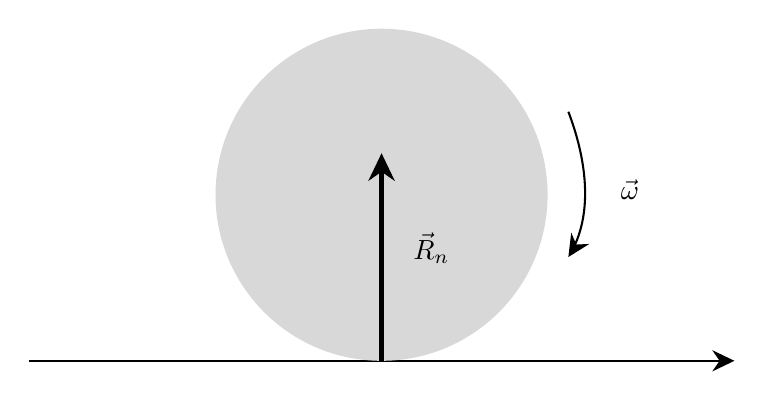
\begin{tikzpicture}[x=0.75pt,y=0.75pt,yscale=-1,xscale=1]
	%uncomment if require: \path (0,300); %set diagram left start at 0, and has height of 300

	%Straight Lines [id:da5764642361967112] 
	\draw    (120,260) -- (457,260) ;
	\draw [shift={(460,260)}, rotate = 180] [fill={rgb, 255:red, 0; green, 0; blue, 0 }  ][line width=0.08]  [draw opacity=0] (10.72,-5.15) -- (0,0) -- (10.72,5.15) -- (7.12,0) -- cycle    ;
	%Shape: Circle [id:dp31649283228684366] 
	\draw  [draw opacity=0][fill={rgb, 255:red, 216; green, 216; blue, 216 }  ,fill opacity=1 ] (210,180) .. controls (210,135.82) and (245.82,100) .. (290,100) .. controls (334.18,100) and (370,135.82) .. (370,180) .. controls (370,224.18) and (334.18,260) .. (290,260) .. controls (245.82,260) and (210,224.18) .. (210,180) -- cycle ;
	%Straight Lines [id:da8430112699742474] 
	\draw [line width=1.5]    (290,260) -- (290,164) ;
	\draw [shift={(290,160)}, rotate = 450] [fill={rgb, 255:red, 0; green, 0; blue, 0 }  ][line width=0.08]  [draw opacity=0] (13.4,-6.43) -- (0,0) -- (13.4,6.44) -- (8.9,0) -- cycle    ;
	%Curve Lines [id:da9237086565736599] 
	\draw    (380,140) .. controls (388.32,161.76) and (392.34,187.82) .. (381.44,207.57) ;
	\draw [shift={(380,210)}, rotate = 302.35] [fill={rgb, 255:red, 0; green, 0; blue, 0 }  ][line width=0.08]  [draw opacity=0] (10.72,-5.15) -- (0,0) -- (10.72,5.15) -- (7.12,0) -- cycle    ;

	% Text Node
	\draw (314,205.67) node    {$\vec{R}_{n}$};
	% Text Node
	\draw (409.67,177.67) node    {$\vec{\omega }$};

	\end{tikzpicture}
\end{figure}